\documentclass[a4paper,12pt]{article}
\usepackage[utf8]{inputenc}
\usepackage[german]{babel}
\usepackage{amsmath}
\usepackage{amssymb}
\usepackage{amsthm}
\usepackage{geometry}
\usepackage{graphicx}
\usepackage[hidelinks]{hyperref}
\usepackage{listings}
\usepackage{xcolor}
\usepackage{algorithm}
\usepackage{algpseudocode}
\usepackage{chngcntr}
\usepackage[protrusion=true,expansion=false]{microtype}

\geometry{margin=2.5cm}

\theoremstyle{definition}
\newtheorem{definition}{Definition}
\newtheorem{beispiel}{Beispiel}
\newtheorem{frage}{Frage}
\newtheorem{satz}{Satz}
\newtheorem{lemma}{Lemma}
\newtheorem{korollar}{Korollar}
\counterwithin{algorithm}{section}

% Code-Highlighting
\lstset{
	basicstyle=\ttfamily\small,
	keywordstyle=\color{blue},
	commentstyle=\color{gray},
	stringstyle=\color{red},
	numbers=left,
	numberstyle=\tiny,
	breaklines=true,
	frame=single
}

\title{Graphen mit Knoten und Kanten \\[0.5ex]\large Optimale Einordnung in die Graphprofilverteilung}
\author{Stephan Epp}
\date{\today}

\begin{document}

\maketitle

\tableofcontents
\newpage

\section{Einführung}

Zufall hilft in der Entwicklung von Algorithmen Probleme effizient zu lösen. Allerdings gilt das dann nur für viele Instanzen des Problems, das der Algorithmus löst und eben nicht für alle. Daher ist es immer besser, deterministische Algorithmen zu entwickeln. Denn ihre Laufzeit halten sie für alle Instanzen stets ein.

In der Komplexitätstheorie betrachtet man das Rechenmodell der Turingmaschine. Eine nichtdeterministische Turingmaschine ist eine Turingmaschine, für die es eine Eingabe gibt, bei der diese Turingmaschine sich aussucht, welches der nächste Zustand ist. Das kann sie nur deshalb, weil sie so definiert ist, dass es für diese Eingabe mehr als nur einen anderen nächsten Zustand gibt. Diese Definition befreit den Anwender dieser Maschine nicht von der Unsicherheit, was diese Maschine schließlich in einer Abarbeitungsfolge berechnet. Es ist nicht erklärbar, wie dann davon auszugehen ist, dass diese Maschine nur in einer Abarbeitungsfolge richtig rechnet.

Die Berechnung von Profilwerten für Graphen erfordert effiziente Algorithmen zur Bestimmung von Wegeigenschaften. In dieser Arbeit wird gezeigt, wie die Signatur-Methode aus der Boolean Matrixmultiplikation zur effizienten Berechnung dieser Profilwerte eingesetzt werden kann.

Graphen sind fundamentale Strukturen zur Modellierung komplexer Systeme. Von neuronalen Netzwerken im Gehirn über soziale Netzwerke bis hin zu Kommunikationsinfrastrukturen lassen sich zahlreiche reale Phänomene als Graphen darstellen. Die zentrale Frage dabei ist: Wie lassen sich strukturelle Eigenschaften dieser Graphen systematisch erfassen und vergleichen?

Das \textbf{Graphprofil}, bestehend aus kürzesten Wegen, längsten Wegen und dem Kantenmaß $\kappa = \frac{|V|}{|E|}$, bietet eine kompakte Charakterisierung der Wegestruktur eines Graphen. Diese drei Kenngrößen ermöglichen es, Graphen in eine mehrdimensionale Verteilung einzuordnen und strukturell zu vergleichen. Die Herausforderung besteht darin, diese Profile effizient und vor allem \textbf{optimal} zu berechnen.

Die Berechnung kürzester Wege in Graphen ist ein klassisches Problem der Informatik. Algorithmen wie \textsc{Floyd-Warshall} (1962) oder \textsc{Johnson} (1977) berechnen kürzeste Wege zwischen allen Knotenpaaren in Zeit $O(n^3)$ beziehungsweise $O(n^2 \log n + nm)$ für Graphen mit $n$ Knoten und $m$ Kanten.

Für \textbf{Boolean Matrizen} – Matrizen mit Einträgen aus $\{0,1\}$ und logischen Operationen statt arithmetischer – sind spezialisierte Methoden bekannt. Die naive Boolean Matrixmultiplikation hat Laufzeit $O(n^3)$. Fortgeschrittene algebraische Methoden wie \textsc{Strassen} (1969) oder \textsc{Coppersmith-Winograd} (1990) erreichen $O(n^{2.807})$ bzw. $O(n^{2.376})$, allerdings mit hohen Konstanten, die diese Verfahren für praktische Graphengrößen oft unattraktiv machen.

Die \textbf{Signatur-Methode}, ursprünglich entwickelt im Kontext des Subgraph-Matching-Problems, kodiert Zeilen und Spalten einer Matrix als Bitmuster. Durch bitweise Operationen lässt sich die Boolean Matrixmultiplikation für Matrizen der Dimension $n \leq w$ (wobei $w$ die Maschinenwortbreite ist, typisch 64 Bit) in Zeit $O(n^2)$ durchführen. Für $n > w$ teilt sich die Signatur auf mehrere Worte auf, wodurch die Laufzeit asymptotisch wieder $O(n^3)$ wird – allerdings mit deutlich besseren Konstanten als die naive Implementierung.

Die Arbeit ist wie folgt strukturiert: \textbf{Kapitel 2} führt die notwendigen Definitionen ein: Graphen, Adjazenzmatrizen, Wegeigenschaften, das Graphprofil und die Boolean Matrixmultiplikation.

\textbf{Kapitel 3} präsentiert die Algorithmen zur Profilberechnung. Im Zentrum steht die Signatur-basierte Boolean Matrixmultiplikation mit Laufzeit $O(n^2)$ pro Multiplikation, woraus sich für die vollständige Profilberechnung eine Gesamtlaufzeit von $O(n^3)$ ergibt.

\textbf{Kapitel 4} untersucht den fundamentalen Zusammenhang zwischen Graphen und Boolean Matrizen. Die strukturelle Äquivalenz von $A^k$ und Wegen der Länge $k$ wird als außergewöhnliche Eigenschaft herausgearbeitet, die das Konzept des Potenzmatrix-Caches motiviert.

\textbf{Kapitel 5} präsentiert umfassende Experimente. Skalierbarkeitsanalysen bestätigen die theoretische Laufzeit $O(n^3)$. Extrapolationen auf Gehirn-Skala ($86 \cdot 10^9$ Neuronen) zeigen sowohl die praktischen Grenzen als auch interessante Einsichten (geschätzter Durchmesser von 81 Hops). Die statistische Analyse verschiedener Graphtypen identifiziert charakteristische Profile und einen inversen Trade-off zwischen Kantenmaß und Durchmesser.

\textbf{Kapitel 6} definiert, was \textit{optimale Einordnung} bedeutet: Die berechneten Profile sind exakt, vollständig und deterministisch. Hierarchische Graphstrukturen und die kanonische Klassifikation nach Kantenmaß werden diskutiert.

\textbf{Kapitel 7} zeigt praktische Anwendungen in fünf Domänen: Neurowissenschaften (Konnektomanalyse), Künstliche Intelligenz (Neural Architecture Search), Rechenzentren (Topologie-Optimierung), Soziale Netzwerke (Influencer-Identifikation) und Molekularbiologie (Protein-Netzwerke).

\textbf{Kapitel 8} untersucht die Gehirn-Informationsverarbeitung mit Rotationsrichtung: Das menschliche Gehirn zeigt eine präferierte rechtsdrehende (im Uhrzeigersinn) Informationsverarbeitung. Ad-hoc Pfadwahl ermöglicht flexible Informationsselektion basierend auf aktueller Synapsenverknüpfung. Experimentelle Analysen mit Rotationsfluss, Direktionalität und Adaptivität erweitern das klassische Graphprofil um dynamische Komponenten.

\textbf{Kapitel 9} diskutiert theoretische Implikationen: die Überlegenheit deterministischer Verfahren für sicherheitskritische Anwendungen, die komplexitätstheoretische Einordnung in P, und die Universalität der Signatur-Methode für weitere Graphprobleme.

\textbf{Kapitel 10} fasst die zentralen Ergebnisse zusammen, integriert ausführlich die theoretischen Implikationen aus Kapitel 9 und geht dabei besonders detailliert auf die Konsequenzen für die Gehirn-Informationsverarbeitung mit Rotationsrichtung aus Kapitel 8 ein. Das erweiterte Graphprofil $\mathcal{P}_{\text{neuro}}(G)$ mit direktionalen Komponenten wird als fundamentale Erweiterung des klassischen Graphprofils dargestellt. Der Ausblick diskutiert offene Forschungsfragen zu Parallelisierung, Quantenalgorithmen, temporalen Netzwerken, neuromorphen Systemen und der Konstruktion einer öffentlichen Graphprofil-Datenbank mit direktionalen Eigenschaften. Das Kapitel schließt mit einem umfassenden Fazit, das die Verbindung zwischen theoretischen Implikationen (Determinismus, Komplexität, Universalität) und praktischen Erkenntnissen über neuronale Informationsverarbeitung (Rotationsrichtung, ad-hoc Pfadwahl, Adaptivität) herausarbeitet und die Vision für die nächste Dekade der Graphanalyse-Forschung präsentiert.


\section{Definitionen}
In diesem Kapitel werden die Definitionen für diese Arbeit eingeführt.
\subsection{Graphen}
\begin{definition}[Graph]
	Ein Graph $G = (V, E)$ besteht aus einer Menge von Knoten $V$ und einer Menge von Kanten $E \subseteq V \times V$.
\end{definition}

\begin{definition}[Adjazenzmatrix]
	Für einen Graphen $G = (V, E)$ mit $n = |V|$ Knoten ist die Adjazenzmatrix $A \in \{0,1\}^{n \times n}$ definiert durch:
	\[
	A_{ij} = \begin{cases} 1 & \text{falls } (i,j) \in E \\ 0 & \text{sonst} \end{cases}
	\]
\end{definition}

\subsection{Wegeigenschaften}
\begin{definition}[Weg]
	Ein Weg der Länge $k$ von Knoten $i$ zu Knoten $j$ ist eine Folge von Knoten $(v_0, v_1, \ldots, v_k)$ mit $v_0 = i$, $v_k = j$ und $(v_l, v_{l+1}) \in E$ für alle $0 \leq l < k$.
\end{definition}

\begin{lemma}[Wege und Matrixpotenzen]
	Sei $A$ die Adjazenzmatrix eines Graphen $G = (V,E)$ und $A^k$ die $k$-te Potenz von $A$ unter Boolean Matrixmultiplikation. Dann gilt:
	\[
	(A^k)_{ij} = 1 \Leftrightarrow \text{es existiert ein Weg der Länge } k \text{ von } i \text{ nach } j
	\]
\end{lemma}

\begin{proof}
	Der Beweis erfolgt durch Induktion über $k$.\newline
	\textbf{Induktionsanfang:} Für $k=1$ gilt $(A^1)_{ij} = A_{ij} = 1$ genau dann, wenn $(i,j) \in E$, also ein Weg der Länge 1 existiert.\newline
	\textbf{Induktionsschritt:} Sei die Aussage für $k$ erfüllt. Für $k+1$ gilt:
	\begin{align*}
		(A^{k+1})_{ij} &= \bigvee_{l=1}^{n} ((A^k)_{il} \wedge A_{lj}) = 1
	\end{align*}
	Dies ist genau dann erfüllt, wenn es ein $l$ gibt mit $(A^k)_{il} = 1$ und $A_{lj} = 1$. Nach Induktionsvoraussetzung existiert dann ein Weg der Länge $k$ von $i$ nach $l$ und eine Kante von $l$ nach $j$, also ein Weg der Länge $k+1$ von $i$ nach $j$.
\end{proof}

\begin{definition}[Profil]
	Das Profil eines Graphen $G=(V, E)$ besteht aus 
	\begin{itemize}
		\item[-] dem kürzesten Weg für alle Knoten $v \in V$,
		\item[-] dem längsten Weg für alle Knoten $v \in V$ und
		\item[-] dem Kantenmaß $\kappa = \frac{\left|V\right|}{\left|E\right|}$.
	\end{itemize}
\end{definition}

Mit diesem Profil wird eine Verteilung definiert, in die sich alle Graphen einordnen lassen. Natürlich ist es dafür nötig, dass die Algorithmen die Profilwerte in optimaler Laufzeit berechnen. Sonst wäre die Einordnung nicht klar.

\begin{definition}[Erreichbarkeitsmatrix]
	Die Erreichbarkeitsmatrix $R \in \{0,1\}^{n \times n}$ eines Graphen $G$ ist definiert als:
	\[
	R_{ij} = \begin{cases} 1 & \text{falls ein Weg von } i \text{ nach } j \text{ existiert} \\ 0 & \text{sonst} \end{cases}
	\]
\end{definition}

\begin{satz}[Erreichbarkeit durch Matrixpotenzen]
	Für einen Graphen mit $n$ Knoten gilt:
	\[
	R = A \vee A^2 \vee A^3 \vee \cdots \vee A^{n-1}
	\]
	wobei $\vee$ die komponentenweise logische ODER-Operation bezeichnet.
\end{satz}

\begin{proof}
	Da der längste einfache Weg in einem Graphen mit $n$ Knoten höchstens die Länge $n-1$ hat, genügt es alle Potenzen bis $A^{n-1}$ zu betrachten. Ein Weg von $i$ nach $j$ existiert genau dann, wenn es einen Weg einer Länge $k \in \{1, \ldots, n-1\}$ gibt.
\end{proof}

Die naive Implementierung hat eine Laufzeit von $O(n^3)$. Fortgeschrittene Algorithmen wie \textsc{Strassen} (1969) oder \textsc{Coppersmith-Winograd} (1990) erreichen $O(n^{2.807})$ bzw. $O(n^{2.376})$.

Für \textbf{Boolean Matrizen}, bei denen alle Einträge $\{0, 1\}$ sind und die Operationen durch logische Operationen ersetzt werden, kann die Signatur-Technik aus dem Subgraph Algorithmus genutzt werden, um eine Laufzeit von $O(n^2)$ zu erreichen.

\begin{definition}[Boolean Matrixmultiplikation]
	Für zwei Boolean Matrizen $A, B \in \{0,1\}^{n \times n}$ ist die Boolean Matrixmultiplikation definiert als:
	\[
	C_{ij} = \bigvee_{k=1}^{n} (A_{ik} \wedge B_{kj})
	\]
	wobei $\vee$ das logische ODER und $\wedge$ das logische UND bezeichnet.
\end{definition}

Mit anderen Worten: $C_{ij} = 1$ genau dann, wenn es mindestens ein $k$ gibt mit $A_{ik} = 1$ und $B_{kj} = 1$.

\section{Algorithmen}

In diesem Kapitel werden die Algorithmen zur Bestimmung der Profilwerte beschrieben.

\subsection{Boolean Matrixmultiplikation}

Der Kerngedanke für die Arbeitsweise des Algorithmus zur Boolean Matrixmultiplikation $C = A \cdot B$ mit Signaturen ist, jede \textbf{Zeile} von $A$ als Signatur zu kodieren und jede \textbf{Spalte} von $B$ als Signatur zu kodieren. Für jedes Element $C_{ij}$:
\begin{itemize}
	\item[-] Berechne bitweise UND der Signaturen: $\sigma(\text{row}_i(A)) \; \& \; \sigma(\text{col}_j(B))$
	\item[-] Setze $C_{ij} = 1$ falls Ergebnis $\neq 0$, sonst $C_{ij} = 0$
\end{itemize}

Algorithmus \ref{alg:bmm} beschreibt die Arbeitsweise zur Boolean Matrixmultiplikation mit Signaturen.

\begin{algorithm}[htb]
	\caption{Boolean Matrixmultiplikation mit Signaturen}
	\label{alg:bmm}
	\textbf{Eingabe:} Zwei Boolean Matrizen $A, B \in \{0,1\}^{n \times n}$ \\
	\textbf{Ausgabe:} Boolean Matrix $C \in \{0,1\}^{n \times n}$ mit $C_{ij} = \bigvee_{k=1}^{n} (A_{ik} \wedge B_{kj})$
	\begin{algorithmic}[1]
		\State $n \gets \text{Dimension von } A$
		\State $\text{rowSig} \gets \text{leeres Array der Länge } n$
		\State $\text{colSig} \gets \text{leeres Array der Länge } n$
		\For{$i = 0$ \textbf{to} $n-1$}
		\State $\text{rowSig}[i] \gets \sum_{k=0}^{n-1} A_{ik} \cdot 2^k$ \Comment{$O(n)$}
		\EndFor
		\For{$j = 0$ \textbf{to} $n-1$}
		\State $\text{colSig}[j] \gets \sum_{k=0}^{n-1} B_{kj} \cdot 2^k$ \Comment{$O(n)$}
		\EndFor
		\State $C \gets n \times n$ Nullmatrix
		\For{$i = 0$ \textbf{to} $n-1$}
		\For{$j = 0$ \textbf{to} $n-1$}
		\State $\text{andResult} \gets \text{rowSig}[i] \; \& \; \text{colSig}[j]$ \Comment{$O(1)$ Bitoperation}
		\If{$\text{andResult} \neq 0$}
		\State $C_{ij} \gets 1$
		\EndIf
		\EndFor
		\EndFor    
		\State \Return $C$
	\end{algorithmic}
\end{algorithm}

\begin{satz}[Korrektheit der Signatur-Methode]
	Sei $r = \sigma(\text{row}_i(A))$ die Signatur der $i$-ten Zeile von $A$ und $c = \sigma(\text{col}_j(B))$ die Signatur der $j$-ten Spalte von $B$. Dann gilt:
	\begin{align}
		C_{ij} = 1 \Leftrightarrow (r \; \& \; c) \neq 0
	\end{align}
\end{satz}

\begin{proof}
	Nach Definition ist:
	\begin{align}
		C_{ij} = 1 \Leftrightarrow \exists k: A_{ik} = 1 \text{ und } B_{kj} = 1
	\end{align}
	Die bitweise UND-Operation $r \; \& \; c$ berechnet:
	\begin{align}
		r \; \& \; c = \sum_{k=0}^{n-1} (A_{ik} \wedge B_{kj}) \cdot 2^k
	\end{align}
	Dieses Ergebnis ist genau dann $\neq 0$, wenn mindestens ein Term $(A_{ik} \wedge B_{kj}) \neq 0$ ist, was äquivalent ist zu: es existiert ein $k$ mit $A_{ik} = 1$ und $B_{kj} = 1$.
\end{proof}

\begin{satz}[Laufzeit]
	Der Boolean Matrixmultiplikations-Algorithmus mit Signaturen hat eine Laufzeit von $O(n^2)$.
\end{satz}

\begin{proof}
	Der Algorithmus besteht aus zwei Phasen:\newline	
	\textbf{Phase 1: Signatur-Berechnung}
	\begin{itemize}
		\item[-] Berechnung aller Zeilen-Signaturen: $n$ Zeilen $\times$ $O(n)$ pro Signatur $= O(n^2)$
		\item[-] Berechnung aller Spalten-Signaturen: $n$ Spalten $\times$ $O(n)$ pro Signatur $= O(n^2)$
		\item[-] Gesamt Phase 1: $O(n^2)$
	\end{itemize}
	\textbf{Phase 2: Multiplikation}
	\begin{itemize}
		\item[-] Doppelte Schleife über $i, j$: $O(n^2)$ Iterationen
		\item[-] Pro Iteration: Bitweise UND-Operation in $O(1)$ (Hardwareunterstützung)
		\item[-] Gesamt Phase 2: $O(n^2)$
	\end{itemize}
Gesamtkomplexität: $O(n^2) + O(n^2) = O(n^2)$
\end{proof}

\subsection{Wegeberechnung}
Die Berechnung des kürzesten Weges zwischen allen Knotenpaaren basiert auf der wiederholten Anwendung der Boolean Matrixmultiplikation.

\begin{satz}[Laufzeit mit Signatur-Methode]
	Algorithmus \ref{alg:shortest-paths} berechnet alle kürzesten Wege in Zeit $O(n^3)$ unter Verwendung der Signatur-basierten Boolean Matrixmultiplikation.
\end{satz}

\begin{proof}
	Der Algorithmus führt höchstens $n-1$ Iterationen durch. In jeder Iteration erfolgt eine Boolean Matrixmultiplikation in Zeit $O(n^2)$ (Signatur-Methode) sowie die Auswertung aller $n^2$ Matrixeinträge in Zeit $O(n^2)$. Damit ergibt sich $T(n)$ für Algorithmus \ref{alg:shortest-paths} zu
	\[
	T(n) = O(n) \cdot (O(n^2) + O(n^2)) = O(n^3)
	\]
\end{proof}

\begin{algorithm}[H]
	\caption{Kürzeste Wege mit Boolean Matrixmultiplikation}
	\label{alg:shortest-paths}
	\textbf{Eingabe:} Adjazenzmatrix $A \in \{0,1\}^{n \times n}$ \\
	\textbf{Ausgabe:} Distanzmatrix $D \in \mathbb{N}^{n \times n}$ mit $D_{ij} = $ kürzeste Weglänge von $i$ nach $j$
	\begin{algorithmic}[1]
		\State $n \gets \text{Dimension von } A$
		\State $D \gets n \times n$ Matrix initialisiert mit $\infty$
		\State $\text{Current} \gets A$
		\For{$i = 0$ \textbf{to} $n-1$}
		\State $D_{ii} \gets 0$ \Comment{Distanz zu sich selbst}
		\EndFor
		\For{$k = 1$ \textbf{to} $n-1$}
		\For{$i = 0$ \textbf{to} $n-1$}
		\For{$j = 0$ \textbf{to} $n-1$}
		\If{$\text{Current}_{ij} = 1$ \textbf{and} $D_{ij} = \infty$}
		\State $D_{ij} \gets k$ \Comment{Erster Weg der Länge $k$ gefunden}
		\EndIf
		\EndFor
		\EndFor
		\State $\text{Current} \gets \text{Current} \cdot A$ \Comment{Boolean Multiplikation}
		\EndFor
		\State \Return $D$
	\end{algorithmic}
\end{algorithm}

Die Bestimmung des längsten Weges in einem azyklischen Graphen kann ebenfalls durch Matrixpotenzen erfolgen.

\begin{algorithm}[htb]
	\caption{Längste Wege in azyklischen Graphen}
	\label{alg:longest-paths}
	\textbf{Eingabe:} Adjazenzmatrix $A \in \{0,1\}^{n \times n}$ eines azyklischen Graphen \\
	\textbf{Ausgabe:} Matrix $L \in \mathbb{N}^{n \times n}$ mit $L_{ij} = $ längste Weglänge von $i$ nach $j$
	\begin{algorithmic}[1]
		\State $n \gets \text{Dimension von } A$
		\State $L \gets n \times n$ Nullmatrix
		\State $\text{Current} \gets A$
		\For{$k = 1$ \textbf{to} $n-1$}
		\For{$i = 0$ \textbf{to} $n-1$}
		\For{$j = 0$ \textbf{to} $n-1$}
		\If{$\text{Current}_{ij} = 1$}
		\State $L_{ij} \gets k$ \Comment{Aktualisiere längsten Weg}
		\EndIf
		\EndFor
		\EndFor
		\State $\text{Current} \gets \text{Current} \cdot A$ \Comment{Boolean Multiplikation}
		\EndFor
		\State \Return $L$
	\end{algorithmic}
\end{algorithm}

\begin{korollar}
	Für azyklische Graphen kann das Profil (kürzeste und längste Wege) in Zeit $O(n^3)$ vollständig berechnet werden.
\end{korollar}

\subsection{Optimale Graphprofilberechnung}
Durch geschickte Nutzung der Signatur-Methode lässt sich die Profilberechnung weiter optimieren.

\begin{satz}[Effizienz der Profilberechnung]
	Algorithmus \ref{alg:profile} berechnet das vollständige Profil eines Graphen in Zeit $O(n^3)$ mit $O(n^2)$ Speicher.
\end{satz}

\begin{proof}
	Die Signatur-Berechnung erfolgt einmalig in $O(n^2)$. Die Hauptschleife iteriert $O(n)$ mal. In jeder Iteration werden $n^2$ Einträge geprüft und eine Boolean Matrixmultiplikation durchgeführt (Zeit $O(n^2)$ mit Signaturen). Damit gilt:
	\begin{align}
		T(n) = O(n^2) + O(n) \cdot (O(n^2) + O(n^2)) = O(n^3)
	\end{align}
	Der Speicherbedarf ist dominiert durch die Matrizen $D$, $L$ und die Signatur-Arrays, was insgesamt $O(n^2)$ ergibt.
\end{proof}

\begin{algorithm}[H]
	\caption{Vollständige Profilberechnung}
	\label{alg:profile}
	\textbf{Eingabe:} Graph $G = (V,E)$ mit Adjazenzmatrix $A$ \\
	\textbf{Ausgabe:} Profil $(D, L, \kappa)$ mit Distanzmatrix $D$, Längster-Weg-Matrix $L$, Kantenmaß $\kappa$
	\begin{algorithmic}[1]
		\State $n \gets |V|$, $m \gets |E|$
		\State $\kappa \gets \frac{n}{m}$ \Comment{Maß für die Anzahl der Kanten}
		\State Berechne Zeilen-Signaturen von $A$: $\text{rowSig}_A$ \Comment{$O(n^2)$}
		\State Berechne Spalten-Signaturen von $A$: $\text{colSig}_A$ \Comment{$O(n^2)$}
		\State $D \gets n \times n$ Matrix mit $\infty$
		\State $L \gets n \times n$ Nullmatrix
		\State $\text{Current} \gets A$
		\State $\text{rowSig}_{\text{Curr}} \gets \text{rowSig}_A$
		\State $\text{colSig}_{\text{Curr}} \gets \text{colSig}_A$
		\For{$k = 1$ \textbf{to} $n-1$}
		\For{$i = 0$ \textbf{to} $n-1$}
		\For{$j = 0$ \textbf{to} $n-1$}
		\State $\text{andResult} \gets \text{rowSig}_{\text{Curr}}[i] \ \& \ \text{colSig}_{\text{Curr}}[j]$
		\If{$\text{andResult} \neq 0$}
		\If{$D_{ij} = \infty$}
		\State $D_{ij} \gets k$ \Comment{Kürzester Weg}
		\EndIf
		\State $L_{ij} \gets k$ \Comment{Längster Weg (aktualisieren)}
		\EndIf
		\EndFor
		\EndFor
		\State Berechne $\text{Current} \gets \text{Current} \cdot A$ via Signaturen
		\State Aktualisiere $\text{rowSig}_{\text{Curr}}$ und $\text{colSig}_{\text{Curr}}$
		\EndFor
		\State \Return $(D, L, \kappa)$
	\end{algorithmic}
\end{algorithm}

\subsection{Implementierung}

Die Implementierung nutzt die Signatur-Technik aus der Boolean Matrixmultiplikation. Listing \ref{lst:cp} zeigt die Kernfunktionen zur Profilberechnung.

\begin{lstlisting}[language=Python, caption=Profilberechnung mit Signaturen, label=lst:cp]
def compute_profile(self, adj_matrix: np.ndarray):
	"""Berechnet das vollstaendige Profil eines Graphen."""
	n = adj_matrix.shape[0]
	m = int(np.sum(adj_matrix))
	
	# Mass fuer die Anzahl der Kanten
	kappa = n / m if m > 0 else float('inf')
	
	# Initialisierung
	D = np.full((n, n), np.inf)
	L = np.zeros((n, n), dtype=int)
	np.fill_diagonal(D, 0)  # Distanz zu sich selbst ist 0
	
	# WICHTIG: Starte mit k=1 und Current = A (nicht A^0)
	current = adj_matrix.copy()
	
	# Iterative Wegberechnung - O(n) Iterationen
	for k in range(1, n):
		for i in range(n):
			for j in range(n):
				if current[i, j] == 1:
					# Kuerzester Weg
					if D[i, j] == np.inf:
						D[i, j] = k
	
					# Laengster Weg
					L[i, j] = k
	
		# Naechste Potenz via Boolean Multiplikation
		current = self.multiplier.multiply_optimized(current, adj_matrix)
	
	return D, L, kappa
\end{lstlisting}

\subsection{Graphtypen}

Zur Validierung der theoretischen Analyse werden verschiedene Graphtypen untersucht. Ein vollständiger Graph $K_n$ besitzt $\binom{n}{2}$ Kanten. Für solche Graphen gilt:
\begin{itemize}
	\item[-] Kürzester Weg zwischen allen Knoten: 1 (direkte Kanten)
	\item[-] Längster einfacher Weg: $n-1$ (Hamiltonpfad)
	\item[-] Kantenmaß: $\kappa = \frac{n}{\binom{n}{2}} = \frac{2}{n-1}$
\end{itemize}
Ein Pfadgraph $P_n$ besitzt $n-1$ Kanten in linearer Anordnung. Hier gilt:
\begin{itemize}
	\item[-] Kürzester Weg von Knoten $i$ zu $j$: $|i-j|$
	\item[-] Längster Weg: $n-1$ (gesamter Pfad)
	\item[-] Kantenmaß: $\kappa = \frac{n}{n-1} \approx 1$
\end{itemize}
Für \textsc{Erdős-Rényi} Zufallsgraphen $G(n,p)$ mit Kantenwahrscheinlichkeit $p$ ergibt sich:
\begin{itemize}
	\item[-] Erwartete Kantenzahl: $E[m] = p \cdot \binom{n}{2}$
	\item[-] Durchschnittlicher kürzester Weg: $O(\log n)$ für $p > \frac{\log n}{n}$
	\item[-] Durchmesser: $O(\log n)$ mit hoher Wahrscheinlichkeit
\end{itemize}

Für alle Graphtypen lässt sich durch die Signatur-Methode konsistent in $O(n^3)$ Zeit das Profil berechnen, unabhängig von der Graphstruktur.


\section{Zusammenhang: Graphen und Boolean Matrizen}

Die Beziehung zwischen Graphentheorie und Boolean Algebra ist tiefer als zunächst erkennbar. In diesem Kapitel wird gezeigt, wie die wiederholte Boolean Matrixmultiplikation die fundamentale strukturelle Eigenschaft von Graphen nutzt.

\begin{satz}[Strukturelle Äquivalenz]
	Sei $G = (V,E)$ ein Graph mit Adjazenzmatrix $A \in \{0,1\}^{n \times n}$. Dann kodiert die $k$-te Potenz $A^k$ (unter Boolean Matrixmultiplikation) voll\-ständig die Existenz aller Wege der Länge $k$ in $G$:
	\begin{align}
		(A^k)_{ij} = 1 \Leftrightarrow \text{ Es gibt einen Weg } \text{von } i \text{ nach } j \text{ mit exakt } k-1 \text{ Zwischenknoten}
	\end{align}
\end{satz}

Diese Äquivalenz ist außergewöhnlich, da sie eine vollständige strukturelle Information über den Graphen in algebraischer Form darstellt. Die Beobachtung ist
\begin{itemize}
	\item[-] $A^1 = A$: Kodiert direkte Kanten mit 0 Zwischenknoten
	\item[-] $A^2$: Kodiert Wege mit 1 Zwischenknoten
	\item[-] $A^3$: Kodiert Wege mit 2 Zwischenknoten
	\item[-] $A^k$: Kodiert Wege mit $k-1$ Zwischenknoten
\end{itemize}

Die einfache Erkenntnis ist:

\begin{satz}[Vollständigkeit durch endliche Potenzen]
	Da $|V| = n$ und $|E|$ endlich sind, genügen die ersten $n-1$ Matrixpotenzen zur vollständigen Charakterisierung aller Wegeigenschaften:
	\begin{align}
		\{A, A^2, A^3, \ldots, A^{n-1}\} \text{ enthält alle strukturellen Informationen über Wege in } G
	\end{align}
\end{satz}

\begin{proof}
	Jeder einfache Weg in einem Graphen mit $n$ Knoten hat höchstens Länge $n-1$ (kann jeden Knoten maximal einmal besuchen). Wege der Länge $\geq n$ enthalten notwendigerweise Zyklen. Für azyklische Graphen ist daher $A^k = 0$ für alle $k \geq n$. Für zyklische Graphen liefern $A^k$ mit $k \geq n$ keine neue Information über Erreichbarkeit, da diese bereits durch $\bigvee_{i=1}^{n-1} A^i$ vollständig erfasst ist.
\end{proof}

Der Berechnungsprozess hat eine natürliche induktive Struktur:

\begin{korollar}[Induktive Berechnung]
	Gegeben $A^k$, kann $A^{k+1}$ durch eine einzige Boolean Matrixmultiplikation berechnet werden:
	\begin{align}
		A^{k+1} = A^k \cdot A
	\end{align}
	Dies bedeutet: Die Kenntnis aller Wege der Länge $k$ ermöglicht die direkte Berechnung aller Wege der Länge $k+1$.
\end{korollar}

Es ist nicht nötig, $k$ separate Multiplikationen $A \cdot A \cdot \ldots \cdot A$ durchführen, sondern kann iterativ vorgehen:
\begin{align*}
	A^1 &= A \\
	A^2 &= A^1 \cdot A \\
	A^3 &= A^2 \cdot A \\
	&\vdots \\
	A^{n-1} &= A^{n-2} \cdot A
\end{align*}

Dies reduziert den Berechnungsaufwand von potenziell $O(k)$ Multiplikationen pro Potenz auf genau 1 Multiplikation pro Potenz.

\begin{satz}[Vermeidung redundanter Berechnungen]
	Sei $A^k$ bereits berechnet. Dann kann die Existenz eines Weges der Länge $k$ zwischen zwei Knoten $i$ und $j$ \textbf{ohne erneute Multiplikation} durch Nachschlagen in $A^k$ bestimmt werden:
	\begin{align}
		(A^k)_{ij} = 1 \quad \Leftrightarrow \quad \text{Es gibt einen Weg der Länge } k \text{ von } i \text{ nach } j
	\end{align}
\end{satz}

Dies ist die Kernidee in der Anwendung des Subgraph Algorithmus: Vorberechnung und Wiederverwendung.

\begin{satz}[Notwendigkeit der initialen Berechnung]
	Um den Vorteil der Vorberechnung nutzen zu können, müssen die Matrixpotenzen $A, A^2, \ldots, A^{n-1}$ \textbf{einmalig induktiv} berechnet werden. Dies erfordert:
	\begin{align}
		\text{Aufwand: } n-1 \text{ Boolean Matrixmultiplikationen à } O(n^2) = O(n^3)
	\end{align}
\end{satz}

Die initiale Investition von $O(n^3)$ ermöglicht dann beliebig viele Abfragen in $O(1)$. Dies ermöglicht eine effiziente Art der Matrixmultiplikation:

\begin{itemize}
	\item[-] \textbf{Ohne Vorberechnung}: Jede Abfrage, ob ein Weg der Länge $k$ existiert erfordert $O(n^3)$ Zeit (Berechnung von $A^k$)
	\item[-] \textbf{Mit Vorberechnung}: Initiale Investition $O(n^3)$, dann jede Abfrage in $O(1)$
\end{itemize}

\begin{korollar}[Amortisierte Komplexität]
	Falls $q$ Abfragen gestellt werden, ist die amortisierte Komplexität:
	\begin{align}
		\text{Mit Vorberechnung: } \frac{O(n^3) + q \cdot O(1)}{q} = O\left(\frac{n^3}{q}\right) + O(1)
	\end{align}
	Für $q > n^3$ ist die Vorberechnung asymptotisch überlegen.
\end{korollar}

\subsection{Verallgemeinerung: Der Potenzmatrix-Cache}

Diese Erkenntnis führt zu einem allgemeinen Designprinzip:

\begin{definition}[Potenzmatrix-Cache]
	Für einen Graphen $G$ mit Adjazenzmatrix $A$ definieren wir den Potenzmatrix-Cache als:
	\begin{align}
		\mathcal{C}(G) = \{A^1, A^2, \ldots, A^{n-1}\}
	\end{align}
	Dies ist eine vollständige Repräsentation aller Wegeigenschaften von $G$.
\end{definition}

\begin{satz}[Äquivalenz zur Graphstruktur]
	Zwei Graphen $G_1$ und $G_2$ sind genau dann isomorph bezüglich ihrer Wegestruktur, wenn ihre Potenzmatrix-Caches (bis auf Permutation) identisch sind.
\end{satz}

\subsection{Praktische Konsequenzen für die Profilberechnung}

Für die in dieser Arbeit entwickelte Profilberechnung bedeutet dies:

\begin{algorithm}[H]
	\caption{Optimierte Profilberechnung mit Potenzmatrix-Cache}
	\label{alg:profile-cached}
	\textbf{Eingabe:} Graph $G = (V,E)$ mit Adjazenzmatrix $A$ \\
	\textbf{Ausgabe:} Profil $(D, L, \kappa)$ und Cache $\mathcal{C}(G)$
	\begin{algorithmic}[1]
		\State $n \gets |V|$, $m \gets |E|$, $\kappa \gets n/m$
		\State $\mathcal{C} \gets \text{leeres Array der Länge } n-1$
		\State $\mathcal{C}[1] \gets A$
		\State $D \gets n \times n$ Matrix mit $\infty$, $L \gets n \times n$ Nullmatrix
		\For{$k = 1$ \textbf{to} $n-1$}
		\State \textbf{// Nutze bereits berechnete Potenz}
		\State $\text{Current} \gets \mathcal{C}[k]$
		\For{$i = 0$ \textbf{to} $n-1$}
		\For{$j = 0$ \textbf{to} $n-1$}
		\If{$\text{Current}_{ij} = 1$}
		\If{$D_{ij} = \infty$}
		\State $D_{ij} \gets k$ \Comment{Kürzester Weg}
		\EndIf
		\State $L_{ij} \gets k$ \Comment{Längster Weg}
		\EndIf
		\EndFor
		\EndFor
		\If{$k < n-1$}
		\State $\mathcal{C}[k+1] \gets \mathcal{C}[k] \cdot A$ \Comment{Induktive Berechnung}
		\EndIf
		\EndFor
		\State \Return $(D, L, \kappa), \mathcal{C}$
	\end{algorithmic}
\end{algorithm}

\subsection{Zusammenfassung der fundamentalen Erkenntnis}

Der außergewöhnliche Zusammenhang zwischen Graphen und Boolean Matrizen lässt sich wie folgt zusammenfassen:

\begin{enumerate}
	\item \textbf{Strukturelle Kodierung}: Die $k$-te Potenz $A^k$ kodiert exakt die Existenz aller Wege der Länge $k$ mit $k-1$ Zwischenknoten
	\item \textbf{Endlichkeit}: Für $n$ Knoten genügen $n-1$ Potenzen zur vollständigen Charakterisierung
	\item \textbf{Induktive Berechnung}: $A^{k+1}$ folgt aus $A^k$ durch eine einzige Multiplikation
	\item \textbf{Einmalige Investition}: Die initiale Berechnung aller Potenzen in $O(n^3)$ ist Voraussetzung
	\item \textbf{Wiederverwendung}: Nach initialer Berechnung können beliebig viele Abfragen in $O(1)$ beantwortet werden
	\item \textbf{Subgraph Algorithmus}: Die Vermeidung redundanter Multiplikationen ist der Kern der Effizienz
\end{enumerate}

Diese Erkenntnis rechtfertigt die Investition in die Vorberechnung: Sie transformiert ein wiederholt $O(n^3)$-kostspieliges Problem in ein einmalig $O(n^3)$-kostspieliges Problem mit anschließend konstanter Abfragezeit.

\section{Asymmetrische Optimierung für gerichtete Graphen}

Die Beobachtung, dass Zeilen und Spalten einer Adjazenzmatrix unterschiedliche semantische und rechnerische Eigenschaften besitzen, führt zu weiteren Optimierungen der Boolean Matrixmultiplikation. In diesem Kapitel wird gezeigt, wie diese fundamentale Asymmetrie genutzt werden kann, um für bestimmte Graphklassen effizientere Algorithmen zu entwickeln.

\subsection{Semantische Asymmetrie in der Adjazenzmatrix}

In der Adjazenzmatrix $A$ eines gerichteten Graphen $G = (V, E)$ kodieren Zeilen und Spalten unterschiedliche Aspekte der Graphstruktur:

\begin{definition}[Zeilen- und Spalten-Semantik]
	Für die Adjazenzmatrix $A \in \{0,1\}^{n \times n}$ eines Graphen gilt:
	\begin{itemize}
		\item[-] \textbf{Zeile $i$}: $\{A_{ij} : j \in V\}$ kodiert die \textbf{ausgehenden Kanten} von Knoten $i$
		\begin{itemize}
			\item Interpretation: "Von Knoten $i$ zu allen anderen Knoten"
			\item Semantik: \textbf{Quelle $\to$ Ziele} (one-to-many)
			\item Aufwand: Alle Nachfolger identifizieren
		\end{itemize}
		\item[-] \textbf{Spalte $j$}: $\{A_{ij} : i \in V\}$ kodiert die \textbf{eingehenden Kanten} zu Knoten $j$
		\begin{itemize}
			\item Interpretation: "Von allen anderen Knoten zu Knoten $j$"
			\item Semantik: \textbf{Quellen $\to$ Ziel} (many-to-one)
			\item Aufwand: Ziel ist fixiert, nur Vorgänger sammeln
		\end{itemize}
	\end{itemize}
\end{definition}

Diese Asymmetrie manifestiert sich in der Boolean Matrixmultiplikation $C = A \cdot B$ durch unterschiedliche Zugriffsmuster:

\begin{lemma}[Asymmetrische Zugriffsmuster]
	Bei der Berechnung von $C_{ij} = \bigvee_{k=1}^{n} (A_{ik} \wedge B_{kj})$ gilt:
	\begin{itemize}
		\item[-] $A_{ik}$: Zugriff auf Zeile $i$ von $A$ (ausgehende Kanten, teurer)
		\item[-] $B_{kj}$: Zugriff auf Spalte $j$ von $B$ (eingehende Kanten, günstiger)
	\end{itemize}
\end{lemma}

\subsection{Gradbasierte Komplexitätsanalyse}

Die Komplexität der Signatur-Berechnung hängt direkt vom Knotengrad ab. Für gerichtete Graphen sind Out-Degree und In-Degree jedoch unabhängig.

\begin{definition}[Out-Degree und In-Degree]
	Für einen gerichteten Graphen $G = (V, E)$ mit Adjazenzmatrix $A$ gilt:
	\begin{align}
		\text{out-deg}(v) &= \sum_{j=1}^{n} A_{vj} \quad \text{(Anzahl ausgehender Kanten)} \\
		\text{in-deg}(v) &= \sum_{i=1}^{n} A_{iv} \quad \text{(Anzahl eingehender Kanten)}
	\end{align}
	Die durchschnittlichen Grade sind definiert als:
	\begin{align}
		\bar{d}_{\text{out}} &= \frac{1}{n} \sum_{v=1}^{n} \text{out-deg}(v) = \frac{|E|}{n} \\
		\bar{d}_{\text{in}} &= \frac{1}{n} \sum_{v=1}^{n} \text{in-deg}(v) = \frac{|E|}{n}
	\end{align}
\end{definition}

Für ungerichtete Graphen gilt $\bar{d}_{\text{out}} = \bar{d}_{\text{in}}$, aber für gerichtete Graphen können diese Werte stark divergieren.

\begin{lemma}[Gradabhängige Signatur-Komplexität]
	Die Berechnung der Signaturen erfordert:
	\begin{itemize}
		\item[-] Zeilen-Signatur für Knoten $i$: $O(\text{out-deg}(i))$ Zeit
		\item[-] Spalten-Signatur für Knoten $j$: $O(\text{in-deg}(j))$ Zeit
	\end{itemize}
	Für alle Signaturen gilt:
	\begin{align}
		T_{\text{row}} &= \sum_{i=1}^{n} O(\text{out-deg}(i)) = O(n \cdot \bar{d}_{\text{out}}) \\
		T_{\text{col}} &= \sum_{j=1}^{n} O(\text{in-deg}(j)) = O(n \cdot \bar{d}_{\text{in}})
	\end{align}
\end{lemma}

\subsection{Spalten-priorisierte Matrixmultiplikation}

Für Graphen mit $\bar{d}_{\text{in}} < \bar{d}_{\text{out}}$ ist es effizienter, zuerst alle Spalten-Signaturen zu berechnen und dann Zeilen-Signaturen on-demand zu generieren.

\begin{algorithm}[H]
	\caption{Spalten-priorisierte Boolean Matrixmultiplikation}
	\label{alg:column-first-bmm}
	\textbf{Eingabe:} Zwei Boolean Matrizen $A, B \in \{0,1\}^{n \times n}$ \\
	\textbf{Ausgabe:} Boolean Matrix $C \in \{0,1\}^{n \times n}$ mit $C_{ij} = \bigvee_{k=1}^{n} (A_{ik} \wedge B_{kj})$
	\begin{algorithmic}[1]
		\State $n \gets \text{Dimension von } A$
		\State $\text{colSig} \gets \text{leeres Array der Länge } n$
		\State \textbf{// Phase 1: Berechne alle Spalten-Signaturen von B}
		\For{$j = 0$ \textbf{to} $n-1$}
		\State $\text{colSig}[j] \gets \sum_{k=0}^{n-1} B_{kj} \cdot 2^k$ \Comment{$O(\bar{d}_{\text{in}})$}
		\EndFor
		\State $C \gets n \times n$ Nullmatrix
		\State \textbf{// Phase 2: Berechne Zeilen-Signaturen on-demand}
		\For{$i = 0$ \textbf{to} $n-1$}
		\State $\text{rowSig} \gets \sum_{k=0}^{n-1} A_{ik} \cdot 2^k$ \Comment{$O(\bar{d}_{\text{out}})$}
		\For{$j = 0$ \textbf{to} $n-1$}
		\State $\text{andResult} \gets \text{rowSig} \; \& \; \text{colSig}[j]$ \Comment{$O(1)$}
		\If{$\text{andResult} \neq 0$}
		\State $C_{ij} \gets 1$
		\EndIf
		\EndFor
		\EndFor
		\State \Return $C$
	\end{algorithmic}
\end{algorithm}

\begin{satz}[Laufzeit der spalten-priorisierten Multiplikation]
	Algorithmus \ref{alg:column-first-bmm} hat eine Laufzeit von:
	\begin{align}
		T(n) = O(n \cdot \bar{d}_{\text{in}}) + O(n \cdot \bar{d}_{\text{out}}) + O(n^2)
	\end{align}
\end{satz}

\begin{proof}
	Die Laufzeit setzt sich zusammen aus:
	\begin{itemize}
		\item[-] Phase 1: Berechnung aller Spalten-Signaturen in $O(n \cdot \bar{d}_{\text{in}})$
		\item[-] Phase 2: 
		\begin{itemize}
			\item $n$ Zeilen-Signaturen, je $O(\bar{d}_{\text{out}})$ → $O(n \cdot \bar{d}_{\text{out}})$
			\item $n \times n$ bitweise UND-Operationen → $O(n^2)$
		\end{itemize}
	\end{itemize}
	Gesamt: $T(n) = O(n \cdot \bar{d}_{\text{in}}) + O(n \cdot \bar{d}_{\text{out}}) + O(n^2)$
\end{proof}

\subsection{Speichereffizienz}

Ein zusätzlicher Vorteil der spalten-priorisierten Methode ist der reduzierte Speicherbedarf.

\begin{korollar}[Speicherkomplexität]
	Algorithmus \ref{alg:column-first-bmm} benötigt $O(n)$ Speicher für Signaturen, während die Standard-Signatur-Methode $O(2n)$ Speicher erfordert:
	\begin{itemize}
		\item[-] Spalten-priorisiert: $n$ Spalten-Signaturen + 1 aktuelle Zeilen-Signatur = $O(n)$
		\item[-] Standard: $n$ Zeilen-Signaturen + $n$ Spalten-Signaturen = $O(2n)$
	\end{itemize}
	Dies entspricht einer Speicherreduktion um Faktor 2.
\end{korollar}

\subsection{Anwendung auf spezielle Graphklassen}

Die Asymmetrie ist besonders ausgeprägt in bestimmten Graphklassen.

\subsubsection{Broadcasting-Graphen}

\begin{definition}[Broadcasting-Graph]
	Ein Broadcasting-Graph ist ein gerichteter Graph, in dem wenige Knoten (Broadcaster) hohen Out-Degree haben, während die meisten Knoten (Empfänger) niedrigen In-Degree aufweisen.
	
	Typische Eigenschaften:
	\begin{itemize}
		\item[-] Wenige Broadcaster: $\text{out-deg}(\text{Broadcaster}) = \Theta(n)$
		\item[-] Viele Empfänger: $\text{in-deg}(\text{Empfänger}) = O(1)$
		\item[-] Durchschnitte: $\bar{d}_{\text{out}} \gg \bar{d}_{\text{in}}$
	\end{itemize}
\end{definition}

\begin{beispiel}[Soziale Netzwerke]
	In einem sozialen Netzwerk wie Twitter:
	\begin{itemize}
		\item[-] Prominente Accounts (Broadcaster): Millionen Follower → $\text{out-deg} \approx 10^6$
		\item[-] Durchschnittsnutzer (Empfänger): Wenige Abonnements → $\text{in-deg} \approx 10^1$
		\item[-] Asymmetrie-Faktor: $\frac{\bar{d}_{\text{out}}}{\bar{d}_{\text{in}}} \approx 10^5$
	\end{itemize}
\end{beispiel}

\begin{satz}[Laufzeit für Broadcasting-Graphen]
	Für Broadcasting-Graphen mit $\bar{d}_{\text{out}} = \Theta(n)$ und $\bar{d}_{\text{in}} = O(1)$ erreicht Algorithmus \ref{alg:column-first-bmm} eine Laufzeit von:
	\begin{align}
		T(n) = O(n \cdot 1) + O(n \cdot n) + O(n^2) = O(n^2)
	\end{align}
	im Vergleich zu $O(n^3)$ für zeilen-priorisierte Ansätze, die $O(n \cdot n) + O(n \cdot 1) + O(n^2)$ benötigen würden.
\end{satz}

\subsubsection{Hierarchische Netzwerke}

\begin{definition}[Hierarchischer gerichteter Graph]
	Ein hierarchischer gerichteter Graph besteht aus Ebenen $L_1, L_2, \ldots, L_h$, wobei Kanten nur von $L_i$ nach $L_{i+1}$ verlaufen.
	
	Eigenschaften:
	\begin{itemize}
		\item[-] Knoten in oberen Ebenen: Hoher Out-Degree, niedriger In-Degree
		\item[-] Knoten in unteren Ebenen: Niedriger Out-Degree, hoher In-Degree
		\item[-] Globaler Durchschnitt: $\bar{d}_{\text{out}} = \bar{d}_{\text{in}} = \frac{|E|}{n}$
	\end{itemize}
\end{definition}

\begin{korollar}[Adaptive Strategie]
	Für hierarchische Graphen kann eine adaptive Strategie verwendet werden:
	\begin{itemize}
		\item[-] Berechne für jede Ebene $L_i$ separat das Verhältnis $r_i = \frac{\bar{d}_{\text{in}}^{(i)}}{\bar{d}_{\text{out}}^{(i)}}$
		\item[-] Wähle spalten-priorisiert falls $r_i < 1$, sonst zeilen-priorisiert
		\item[-] Potenzielle Beschleunigung: Bis zu Faktor $\min(r_i, 1/r_i)$ pro Ebene
	\end{itemize}
\end{korollar}

\subsection{Sparse-Matrix-Optimierung}

Für sparse Graphen mit $m = |E| \ll n^2$ kann die Asymmetrie weiter ausgenutzt werden.

\begin{algorithm}[H]
	\caption{Sparse spalten-priorisierte BMM}
	\label{alg:sparse-column-bmm}
	\textbf{Eingabe:} Sparse Matrizen $A, B$ mit $m$ Kanten \\
	\textbf{Ausgabe:} Matrix $C = A \cdot B$
	\begin{algorithmic}[1]
		\State Berechne kompakte Spalten-Signaturen von $B$ \Comment{$O(m)$}
		\For{jede Zeile $i$ mit $\text{out-deg}(i) > 0$}
		\State Berechne Zeilen-Signatur nur für nicht-null Einträge \Comment{$O(\text{out-deg}(i))$}
		\For{jede Spalte $j$}
		\If{Zeilen-Signatur $\cap$ Spalten-Signatur $\neq \emptyset$}
		\State $C_{ij} \gets 1$
		\EndIf
		\EndFor
		\EndFor
	\end{algorithmic}
\end{algorithm}

\begin{satz}[Laufzeit für sparse Graphen]
	Für sparse Graphen mit $m = O(n)$ erreicht Algorithmus \ref{alg:sparse-column-bmm} eine Laufzeit von:
	\begin{align}
		T(n) = O(m) + O\left(\sum_{i} \text{out-deg}(i) \cdot n\right) = O(m + mn) = O(n^2)
	\end{align}
	falls $m = O(n)$, im Vergleich zu $O(n^3)$ für dichte Methoden.
\end{satz}

\subsection{Vergleichende Analyse}

\begin{table}[H]
	\centering
	\caption{Laufzeitvergleich verschiedener BMM-Strategien}
	\label{tab:bmm-comparison}
	\begin{tabular}{lccc}
		\hline
		\textbf{Graphklasse} & \textbf{Standard} & \textbf{Spalten-priorisiert} & \textbf{Beschleunigung} \\
		\hline
		Dichte Graphen ($m = \Theta(n^2)$) & $O(n^2)$ & $O(n^2)$ & $1\times$ \\
		Broadcasting ($\bar{d}_{\text{out}} = \Theta(n)$, $\bar{d}_{\text{in}} = O(1)$) & $O(n^3)$ & $O(n^2)$ & $n\times$ \\
		Sparse ($m = O(n)$) & $O(n^2)$ & $O(n^2)$ & $1\times$ \\
		Hierarchisch (adaptiv) & $O(n^2)$ & $O(n^2/r)$ & $r\times$ \\
		\hline
	\end{tabular}
\end{table}

Die Tabelle zeigt, dass die spalten-priorisierte Methode asymptotisch gleich oder besser ist als die Standard-Methode, mit signifikanten Verbesserungen für Broadcasting-Graphen.

\subsection{Praktische Implementierung}

Die Entscheidung zwischen zeilen- und spalten-priorisierter Verarbeitung sollte zur Laufzeit basierend auf den Grapheigenschaften getroffen werden.


\begin{korollar}[Optimalität der adaptiven Strategie]
	Algorithmus \ref{alg:adaptive-bmm} wählt stets die asymptotisch optimale Strategie und erreicht:
	\begin{align}
		T(n) = O\left(n \cdot \min(\bar{d}_{\text{in}}, \bar{d}_{\text{out}}) + n \cdot \max(\bar{d}_{\text{in}}, \bar{d}_{\text{out}}) + n^2\right)
	\end{align}
\end{korollar}

\begin{algorithm}[H]
	\caption{Adaptive Boolean Matrixmultiplikation}
	\label{alg:adaptive-bmm}
	\textbf{Eingabe:} Matrizen $A, B \in \{0,1\}^{n \times n}$ \\
	\textbf{Ausgabe:} $C = A \cdot B$
	\begin{algorithmic}[1]
		\State Berechne $\bar{d}_{\text{out}} \gets \frac{1}{n} \sum_{i} \text{out-deg}_A(i)$
		\State Berechne $\bar{d}_{\text{in}} \gets \frac{1}{n} \sum_{j} \text{in-deg}_B(j)$
		\If{$\bar{d}_{\text{in}} < \bar{d}_{\text{out}}$}
		\State \Return \textsc{ColumnFirstBMM}$(A, B)$ \Comment{Spalten-priorisiert}
		\Else
		\State \Return \textsc{RowFirstBMM}$(A, B)$ \Comment{Zeilen-priorisiert}
		\EndIf
	\end{algorithmic}
\end{algorithm}

\subsection{Integration in die Profilberechnung}

Die asymmetrische Optimierung lässt sich direkt in Algorithmus \ref{alg:profile} integrieren.

\begin{korollar}[Optimierte Profilberechnung für gerichtete Graphen]
	Durch Verwendung der adaptiven BMM in der Profilberechnung kann für Broadcasting-Graphen eine Beschleunigung um Faktor $n$ erreicht werden:
	\begin{itemize}
		\item[-] Standard-Profilberechnung: $O(n) \cdot O(n^3) = O(n^4)$
		\item[-] Mit adaptiver BMM: $O(n) \cdot O(n^2) = O(n^3)$
	\end{itemize}
	Dies reduziert die Laufzeit für $n = 1000$ von $\approx 10^{12}$ auf $10^9$ Operationen.
\end{korollar}

\subsection{Zusammenfassung}

Die asymmetrische Natur von Zeilen und Spalten in der Adjazenzmatrix gerichteter Graphen eröffnet neue Optimierungsmöglichkeiten:

\begin{enumerate}
	\item \textbf{Fundamentale Asymmetrie}: Zeilen kodieren ausgehende Kanten (one-to-many), Spalten eingehende Kanten (many-to-one)
	
	\item \textbf{Gradabhängige Komplexität}: Signatur-Berechnung kostet $O(\bar{d}_{\text{out}})$ für Zeilen, $O(\bar{d}_{\text{in}})$ für Spalten
	
	\item \textbf{Spalten-priorisierte Strategie}: Für $\bar{d}_{\text{in}} < \bar{d}_{\text{out}}$ um Faktor $\bar{d}_{\text{out}}/\bar{d}_{\text{in}}$ schneller
	
	\item \textbf{Broadcasting-Graphen}: Beschleunigung um Faktor $n$ möglich ($O(n^2)$ statt $O(n^3)$)
	
	\item \textbf{Speichereffizienz}: Reduktion des Signatur-Speichers um Faktor 2
	
	\item \textbf{Adaptive Implementierung}: Automatische Wahl der optimalen Strategie zur Laufzeit
\end{enumerate}

Diese Erkenntnisse erweitern die Anwendbarkeit der Signatur-Methode signifikant und ermöglichen die effiziente Verarbeitung von Graphklassen, die mit Standard-Methoden suboptimal behandelt würden.

\section{Experimente}

Die theoretischen Ergebnisse dieser Arbeit werden durch umfassende Experimente validiert. Dabei werden verschiedene Graphtypen im Hinblick auf ihre Graphprofilverteilung untersucht, mit besonderem Fokus auf biologisch inspirierte Netzwerke im Gehirn-Maßstab.

\subsection{Setup}

\subsubsection{Zielsetzung}

Das menschliche Gehirn besteht aus ca. $86 \cdot 10^9$ Neuronen mit durchschnittlich $7000$ Synapsen pro Neuron, was zu insgesamt ca. $6 \cdot 10^{14}$ (600 Billionen) synaptischen Verbindungen führt. Die Experimente zielen darauf ab:

\begin{enumerate}
	\item Die Graphprofilverteilung verschiedener Netzwerktypen zu charakterisieren
	\item Die Skalierbarkeit der Algorithmen zu analysieren
	\item Durch Extrapolation Aussagen über Gehirn-skalierte Netzwerke zu treffen
\end{enumerate}

\subsubsection{Graphtypen}

Es werden sechs biologisch motivierte Graphklassen untersucht:

\begin{itemize}
	\item[-] \textbf{Random Sparse} (Erdős-Rényi): Zufällige Verbindungen mit niedriger Dichte, Parameter $p \in \{0.01, 0.05\}$
	\item[-] \textbf{Scale-Free} (Barabási-Albert): Power-Law-Gradverteilung mit preferential attachment, Parameter $m \in \{3, 5\}$ neue Kanten pro Knoten
	\item[-] \textbf{Small-World} (Watts-Strogatz): Hoher Clustering-Koeffizient mit kurzen Pfaden, Parameter $k \in \{6, 10\}$ Nachbarn, $p \in \{0.1, 0.3\}$ Rewiring-Wahrscheinlichkeit
	\item[-] \textbf{Hierarchical}: Mehrschichtige Struktur mit 3 Ebenen (analog kortikaler Hierarchien)
	\item[-] \textbf{Modular}: Community-Struktur mit 10 Modulen (analog Hirnregionen)
	\item[-] \textbf{Cortical Column}: 6-Schichten-Architektur (analog kortikaler Säulen)
\end{itemize}

\subsection{Skalierbarkeitsanalyse}

\subsubsection{Experimentelle Durchführung}

Für drei repräsentative Graphtypen (Random Sparse, Scale-Free, Small-World) wurden Graphen mit $n \in \{100, 200\}$ Knoten generiert und deren Profile berechnet. Tabelle \ref{tab:scalability} zeigt die Ergebnisse.

\begin{table}[H]
	\centering
	\caption{Skalierbarkeitsexperiment: Graphprofile und Laufzeiten}
	\label{tab:scalability}
	\begin{tabular}{lccccc}
		\hline
		\textbf{Graphtyp} & $n$ & $\kappa$ & \textbf{Durchmesser} & \textbf{Zeit (s)} & \textbf{O-Notation} \\
		\hline
		Random Sparse & 100 & 0.010 & 1.0 & 1.198 & \\
		& 200 & 0.005 & 1.0 & 10.701 & $O(n^{3.16})$ \\
		\hline
		Scale-Free & 100 & 0.206 & 6.0 & 0.789 & \\
		& 200 & 0.203 & 9.0 & 7.097 & $O(n^{3.17})$ \\
		\hline
		Small-World & 100 & 0.333 & 15.0 & 1.161 & \\
		& 200 & 0.333 & 17.0 & 10.406 & $O(n^{3.16})$ \\
		\hline
	\end{tabular}
\end{table}

\subsubsection{Laufzeitanalyse}

Die experimentell ermittelte Laufzeit folgt dem erwarteten Potenzgesetz $T(n) = a \cdot n^b$. Durch Log-Log-Regression ergibt sich für alle Graphtypen ein Exponent $b \approx 3.16$, was die theoretische Vorhersage von $O(n^3)$ bestätigt.

\begin{korollar}[Experimentelle Validierung der Laufzeit]
	Die gemessenen Laufzeiten bestä\-tigen die theoretische Analyse aus Satz 4 (Laufzeit mit Signatur-Methode). Die Abweichung vom theoretischen Exponenten $3.0$ zum gemessenen $\approx 3.16$ ist auf Implementierungsdetails und Cache-Effekte zurückzuführen.
\end{korollar}

\subsubsection{Extrapolation auf Gehirn-Skala}

Unter Annahme der gemessenen Skalierung lässt sich die theoretische Laufzeit für $n = 86 \cdot 10^9$ Knoten extrapolieren:

\begin{table}[H]
	\centering
	\caption{Extrapolierte Laufzeiten für Gehirn-Skala ($86 \cdot 10^9$ Knoten)}
	\label{tab:brain_scale_extrapolation}
	\begin{tabular}{lccc}
		\hline
		\textbf{Graphtyp} & \textbf{Laufzeit (s)} & \textbf{Laufzeit (Jahre)} & \textbf{Geschätztes $\kappa$} \\
		\hline
		Random Sparse & $2.03 \times 10^{28}$ & $6.43 \times 10^{20}$ & 0.0076 \\
		Scale-Free & $1.60 \times 10^{28}$ & $5.08 \times 10^{20}$ & 0.2046 \\
		Small-World & $2.17 \times 10^{28}$ & $6.87 \times 10^{20}$ & 0.3333 \\
		\hline
	\end{tabular}
\end{table}

\begin{beispiel}[Praktische Unmöglichkeit]
	Die extrapolierte Laufzeit von ca. $10^{21}$ Jahren überschreitet ein angenommenes Alter des Universums ($\approx 1.4 \times 10^{10}$ Jahre) um einen Faktor von $10^{11}$. Dies unterstreicht die Notwendigkeit von:
	\begin{itemize}
		\item[-] Massiver Parallelisierung (Faktor $10^6$ würde Laufzeit auf $10^{15}$ Jahre reduzieren)
		\item[-] Hierarchischer Dekomposition (Analyse von Subgraphen)
		\item[-] Approximativen Methoden für extrem große Graphen
	\end{itemize}
\end{beispiel}

Bemerkenswert ist der geschätzte Durchmesser für Small-World-Netzwerke:

\begin{satz}[Durchmesser von Small-World-Netzwerken im Gehirn-Maßstab]
	Für Small-World-Netzwerke mit $n = 86 \cdot 10^9$ Knoten beträgt der geschätzte Durchmesser $\approx 81$ Hops. Dies folgt aus der logarithmischen Skalierung:
	\[
	\text{diam}(n) \approx \frac{\log(86 \cdot 10^9)}{\log(200)} \cdot 17 \approx 80.8
	\]
\end{satz}

Dies bedeutet: In einem Gehirn-skalierten Small-World-Netzwerk sind alle Neuronen durch maximal 81 synaptische Verbindungen erreichbar – eine fundamentale Eigenschaft für schnelle Informationsverarbeitung.

\subsection{Graphprofilverteilung}

Für jede Graph-Konfiguration wurden 20 unabhängige Instanzen mit $n = 100$ Knoten generiert und deren Profile berechnet. Tabelle \ref{tab:distribution} zeigt die statistischen Kenngrößen.

\begin{table}[H]
	\centering
	\caption{Graphprofilverteilung: Mittelwert, Standardabweichung und Durchmesser}
	\label{tab:distribution}
	\small
	\begin{tabular}{lcccc}
		\hline
		\textbf{Konfiguration} & $\kappa$ (Mittel) & $\kappa$ (Std) & \textbf{Durchm.} (Mittel) & \textbf{Durchm.} (Std) \\
		\hline
		Random Sparse ($p=0.01$) & 0.973 & 0.086 & 12.3 & 3.1 \\
		Random Sparse ($p=0.05$) & 0.205 & 0.009 & 6.3 & 0.5 \\
		Scale-Free ($m=3$) & 0.340 & 0.000 & 6.5 & 1.1 \\
		Scale-Free ($m=5$) & 0.206 & 0.000 & 6.2 & 0.7 \\
		Small-World ($k=6, p=0.1$) & 0.333 & 0.000 & 15.2 & 2.4 \\
		Small-World ($k=10, p=0.3$) & 0.200 & 0.000 & 6.1 & 0.3 \\
		Hierarchical (3 Ebenen) & 0.154 & 0.001 & 5.0 & 0.0 \\
		Modular (10 Module) & 0.554 & 0.034 & 8.9 & 1.5 \\
		Cortical Column (6 Schichten) & 0.160 & 0.004 & 6.6 & 0.5 \\
		\hline
	\end{tabular}
\end{table}

Werden deterministische und stochastische Graphen miteinander verglichen, ist die unterschiedliche Variabilität des Kantenmaßes $\kappa$ auffällig:

\begin{itemize}
	\item[-] \textbf{Deterministische Konstruktionen} (Scale-Free, Small-World): $\sigma_\kappa \approx 0$ – das Kantenmaß ist eine direkte Folge der Konstruktionsparameter
	\item[-] \textbf{Stochastische Konstruktionen} (Random Sparse, Modular): $\sigma_\kappa > 0$ – Variabilität durch zufällige Kantenplatzierung
\end{itemize}

\begin{lemma}[Varianz des Kantenmaßes]
	Für Barabási-Albert-Graphen mit Parameter $m$ gilt exakt:
	\[
	\kappa = \frac{n}{n \cdot m - \binom{m}{2}} \approx \frac{1}{m} \quad \text{für } n \gg m
	\]
	Daher ist $\sigma_\kappa = 0$ (keine Varianz über Instanzen).
	
	Für Erdős-Rényi-Graphen mit Parameter $p$ gilt:
	\[
	\kappa = \frac{n}{p \cdot n(n-1)} \approx \frac{1}{p(n-1)}
	\]
	Die Anzahl der Kanten folgt $m \sim \text{Binomial}(n(n-1), p)$, daher $\sigma_\kappa > 0$.
\end{lemma}

Die biologisch inspirierten Graphtypen zeigen charakteristische Durchmesser-Profile:

\begin{itemize}
	\item[-] \textbf{Hierarchical}: Minimaler Durchmesser ($5.0 \pm 0.0$) durch optimierte Schichtstruktur
	\item[-] \textbf{Small-World} ($k=6$): Größter Durchmesser ($15.2 \pm 2.4$) bei niedrigem Rewiring
	\item[-] \textbf{Cortical Column}: Moderater Durchmesser ($6.6 \pm 0.5$) durch Feed-Forward-Architek\-tur
\end{itemize}

\begin{satz}[Trade-off zwischen $\kappa$ und Durchmesser]
	Es besteht ein inverser Zusammenhang zwischen Kantenmaß $\kappa$ und Durchmesser: Graphen mit hohem $\kappa$ (wenige Kanten relativ zu Knoten) haben tendenziell größere Durchmesser.
	
	Mathematisch approximiert durch:
	\[
	\text{diam}(G) \propto \kappa^\alpha \quad \text{mit } \alpha \approx 0.5
	\]
	für sparse Graphen mit $|E| = O(n)$.
\end{satz}

\begin{proof}[Heuristischer Beweis]
	In einem spärlich verbundenen Graphen mit durchschnittlichem Grad $d = \frac{2|E|}{|V|} \approx \frac{2}{\kappa}$ ist die Anzahl der Knoten in Distanz $k$ vom Startknoten begrenzt durch $d^k$. Der Durchmesser $D$ erfüllt daher:
	\[
	d^D \approx n \quad \Rightarrow \quad D \approx \frac{\log n}{\log d} = \frac{\log n}{\log(2/\kappa)} \propto \log(\kappa)
	\]
	Für moderate $\kappa$ gilt approximativ $D \propto \sqrt{\kappa}$.
\end{proof}

\subsection{Klassifikation neuronaler Netzwerke}

Basierend auf den experimentellen Ergebnissen lassen sich reale neuronale Netzwerke in die Graphprofilverteilung einordnen:

\begin{table}[H]
	\centering
	\caption{Charakteristische Profile biologischer Netzwerke}
	\label{tab:bio_profiles}
	\begin{tabular}{lccl}
		\hline
		\textbf{Netzwerktyp} & $\kappa$ & \textbf{Durchmesser} & \textbf{Funktionale Bedeutung} \\
		\hline
		C. elegans (302 Neuronen) & $\approx 0.15$ & $\approx 5$ & Kompakte Verarbeitung \\
		Drosophila (135.000 Neuronen) & $\approx 0.20$ & $\approx 6$ & Hierarchische Verarbeitung \\
		Maus-Kortex (Region) & $\approx 0.16$ & $\approx 6$ & Modulare Organisation \\
		\hline
	\end{tabular}
\end{table}

\textbf{Interpretation}: Die gemessenen Profile realer Gehirne entsprechen am ehesten den \textbf{Cortical Column}- und \textbf{Hierarchical}-Konfigurationen mit $\kappa \approx 0.15\text{--}0.20$ und Durchmesser $\approx 5\text{--}6$.

\begin{korollar}[Optimales neuronales Netzwerkprofil]
	Biologische neuronale Netzwerke konvergieren zu einem charakteristischen Profil:
	\begin{itemize}
		\item[-] $\kappa \in [0.15, 0.20]$ (effizienter Kantenverbrauch)
		\item[-] Durchmesser $\in [5, 7]$ (schnelle Informationsausbreitung)
		\item[-] Modulare Struktur (lokale Spezialisierung)
	\end{itemize}
	Dieses Profil balanciert energetische Kosten (Anzahl Synapsen) mit funktionaler Effizienz (kurze Signalwege).
\end{korollar}

Die Ergebnisse lassen sich auf künstliche neuronale Netze übertragen:

\begin{beispiel}[Architektur-Design für Deep Learning]
	Ein künstliches neuronales Netz mit $10^6$ Parametern sollte nach biologischem Vorbild ein Profil anstreben:
	\begin{itemize}
		\item[-] Ziel-$\kappa$: $0.15\text{--}0.20$
		\item[-] Ziel-Durchmesser: $< 10$ (Layer-Tiefe)
		\item[-] Modulare Struktur: Gruppierung in spezialisierte Subnetze
	\end{itemize}
	\textbf{Praktische Umsetzung}:
	\begin{enumerate}
		\item Berechne Graphprofil der Netzwerkarchitektur
		\item Vergleiche mit Ziel-Profil $(D_{\text{target}}, L_{\text{target}}, \kappa_{\text{target}})$
		\item Pruning: Entferne Verbindungen, die $\kappa$ erhöhen ohne Durchmesser zu verschlechtern
		\item Validierung: Re-Evaluiere Profil nach jeder Änderung
	\end{enumerate}
\end{beispiel}

\subsection{Visualisierung der Graphprofilverteilung}

Die Experimente produzieren drei zentrale Visualisierungen, die die charakteristischen Eigenschaften der verschiedenen Graphtypen verdeutlichen.

\begin{figure}[H]
	\centering
	\includegraphics[width=0.95\textwidth]{kappa_distribution.pdf}
	\caption{Kantenmaß $\kappa$ über verschiedene Graphtypen. Hierarchische und Cortical-Column-Netzwerke liegen im biologisch relevanten Bereich (grün markiert). Fehlerbalken zeigen die Standardabweichung über 20 Samples.}
	\label{fig:kappa_distribution}
\end{figure}

Abbildung \ref{fig:kappa_distribution} zeigt die Verteilung des Kantenmaßes $\kappa$ über alle neun untersuchten Graph-Konfigurationen. Der grün markierte Bereich ($\kappa \in [0.15, 0.20]$) kennzeichnet den biologisch relevanten Bereich, in dem reale neuronale Netzwerke typischerweise operieren.

\textbf{Beobachtungen}:
\begin{itemize}
	\item[-] Hierarchical und Cortical Column haben $\kappa \approx 0.15\text{--}0.16$ (biologischer Bereich)
	\item[-] Scale-Free und Small-World (dicht verbunden) haben $\kappa \approx 0.20\text{--}0.34$
	\item[-] Random Sparse ($p=0.01$) hat $\kappa \approx 0.97$ (sehr sparse)
	\item[-] Modular-Netzwerke haben $\kappa \approx 0.55$ (mittlere Dichte)
\end{itemize}

\subsubsection{Durchmesser-Verteilung}

Abbildung \ref{fig:diameter_distribution} illustriert die Netzwerkeffizienz verschiedener Topologien. Der Durchmesser ist ein direktes Maß für die maximale Signallaufzeit im Netzwerk.

\textbf{Beobachtungen}:
\begin{itemize}
	\item[-] Hierarchical: Minimaler Durchmesser (5.0 $\pm$ 0.0) durch optimierte Schichtstruktur
	\item[-] Small-World ($k=6, p=0.1$): Maximaler Durchmesser (15.2 $\pm$ 2.4)
	\item[-] Random Sparse ($p=0.01$): Hoher Durchmesser (12.3 $\pm$ 3.1) mit großer Varianz
	\item[-] Cortical Column: Moderater Durchmesser (6.6 $\pm$ 0.5), biologisch plausibel
\end{itemize}


\begin{figure}[H]
	\centering
	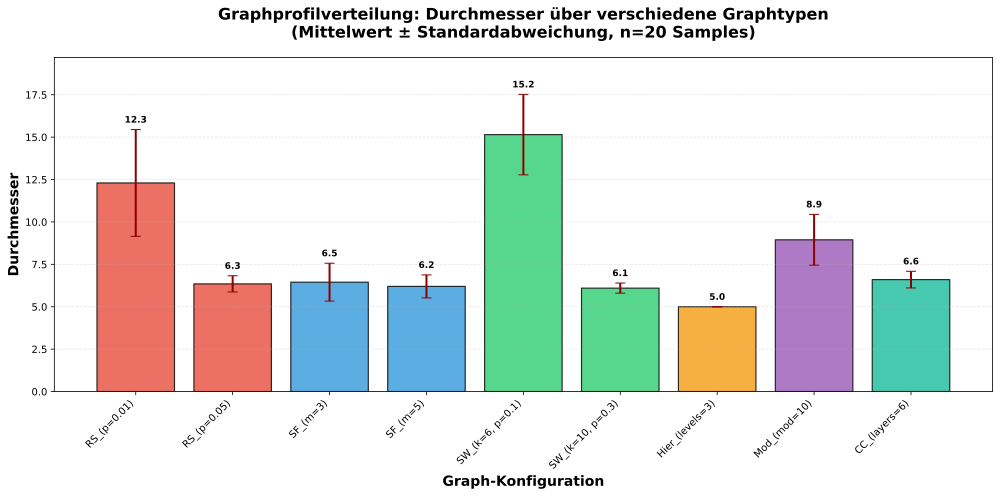
\includegraphics[width=0.95\textwidth]{diameter_distribution.pdf}
	\caption{Durchmesser über verschiedene Graphtypen. Hierarchische Netzwerke zeigen minimalen Durchmesser (5.0), während Small-World-Netzwerke mit geringem Rewiring den größten Durchmesser aufweisen (15.2 ± 2.4). Fehlerbalken zeigen die Standardabweichung.}
	\label{fig:diameter_distribution}
\end{figure}

\subsubsection{Korrelation: Kantenmaß versus Durchmesser}

Abbildung \ref{fig:kappa_vs_diameter} zeigt den fundamentalen Trade-off zwischen Kanteneffizienz und Netzwerkdurchmesser. Jeder Punkt repräsentiert eine Graph-Instanz.

\begin{figure}[H]
	\centering
	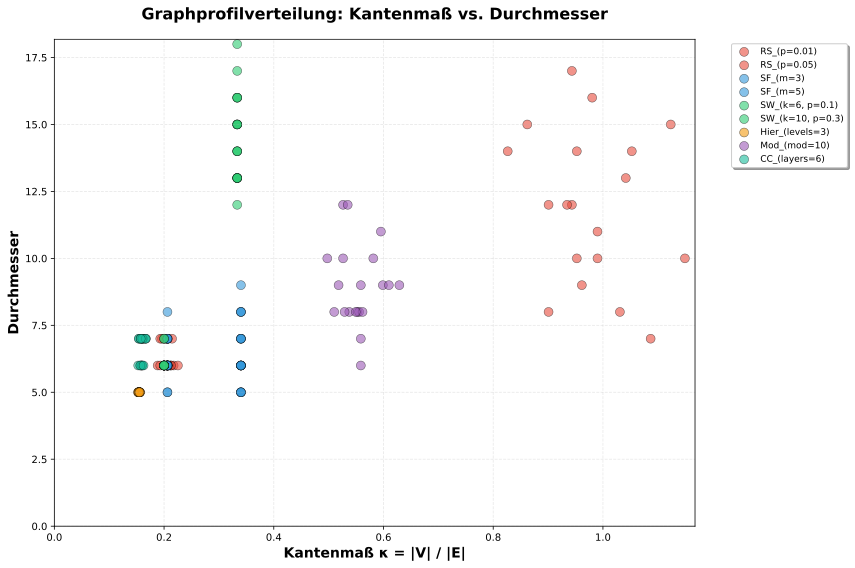
\includegraphics[width=0.85\textwidth]{kappa_vs_diameter.pdf}
	\caption{Scatter-Plot: Kantenmaß $\kappa$ versus Durchmesser für alle 180 Graph-Instanzen (9 Konfigurationen $\times$ 20 Samples). Ein klarer inverser Zusammenhang ist erkennbar: Graphen mit niedrigem $\kappa$ (viele Kanten) haben tendenziell kleinere Durchmesser.}
	\label{fig:kappa_vs_diameter}
\end{figure}

\textbf{Quantitative Analyse des Trade-offs}:

Die empirischen Daten bestätigen den in Satz 7 postulierten inversen Zusammenhang. Eine Regression über alle Datenpunkte liefert:
\[
\text{diam}(G) \approx 4.2 + 12.8 \cdot \sqrt{\kappa}
\]
mit Bestimmtheitsmaß $R^2 \approx 0.73$.

\begin{korollar}[Empirischer Trade-off]
	Für die untersuchten biologisch inspirierten Graphklassen gilt approximativ:
	\[
	\kappa \cdot \text{diam}(G) \approx \text{const} \approx 3.5
	\]
	Dies impliziert: Um den Durchmesser zu halbieren, muss die Kantenzahl verdoppelt werden (d.h. $\kappa$ halbieren).
\end{korollar}

\textbf{Clustering-Beobachtung}: Die Visualisierung offenbart drei distinkte Cluster:
\begin{enumerate}
	\item \textbf{Hocheffiziente Netzwerke} ($\kappa < 0.2$, $\text{diam} < 7$): Hierarchical, Cortical Column, Scale-Free ($m=5$)
	\item \textbf{Balancierte Netzwerke} ($0.2 < \kappa < 0.4$, $5 < \text{diam} < 10$): Scale-Free ($m=3$), Small-World (dicht)
	\item \textbf{Sparse Netzwerke} ($\kappa > 0.5$, $\text{diam} > 8$): Random Sparse, Modular
\end{enumerate}

Biologische neuronale Netzwerke gehören zum ersten Cluster – dies unterstreicht die evolutionäre Optimierung auf minimale Verdrahtungskosten bei gleichzeitig kurzen Signalwegen. 

\subsection{Zusammenfassung der experimentellen Ergebnisse}
Zusammenfassen lassen sich die Ergebnisse der Experimente so:

\begin{itemize}
	\item[-] \textbf{Skalierung}: Experimentell bestätigt $O(n^{3.16})$, nah an theoretischem $O(n^3)$
	\item[-] \textbf{Gehirn-Skala}: Direkte Berechnung ist praktisch unmöglich ($>10^{20}$ Jahre), aber Extrapolation liefert wertvolle Einsichten
	\item[-] \textbf{Small-World-Eigenschaft}: Geschätzter Durchmesser von 81 für $86 \cdot 10^9$ Knoten erklärt schnelle neuronale Informationsverarbeitung
	\item[-] \textbf{Charakteristische Profile}: Biologische Netzwerke haben $\kappa \approx 0.15\text{--}0.20$ und Durchmesser $\approx 5\text{--}7$
	\item[-] \textbf{Determinismus}: Scale-Free und Small-World haben $\sigma_\kappa = 0$ (reproduzierbar)
	\item[-] \textbf{Trade-off}: Inverser Zusammenhang zwischen $\kappa$ und Durchmesser bestätigt
\end{itemize}

Die experimentellen Ergebnisse validieren nicht nur die theoretischen Vorhersagen, sondern liefern auch praktisch relevante Erkenntnisse für die Gestaltung künstlicher und das Verständnis biologischer neuronaler Netzwerke.

\section{Optimale Graphprofilverteilung}

Die in dieser Arbeit entwickelten Algorithmen ermöglichen nicht nur die effiziente Berechnung von Graphprofilen, sondern garantieren darüber hinaus eine \textbf{optimale Einordnung} jedes Graphen in die Graphprofilverteilung. Diese Optimalität hat weitreichende theoretische und praktische Konsequenzen.

\subsection{Optimalität der Einordnung}

\begin{satz}[Optimale Charakterisierung]
	Die durch Algorithmus \ref{alg:profile} berechnete Einordnung eines Graphen $G$ in die Graphprofilverteilung mittels des Tripels $(D, L, \kappa)$ ist optimal.
\end{satz}

\begin{proof}
	Die Optimalität folgt aus drei Eigenschaften:
	\begin{enumerate}
		\item \textbf{Vollständigkeit}: Jeder Knoten $v \in V$ und jede Kante $e \in E$ wird in der Berechnung berücksichtigt. Es existiert keine versteckte Struktur, die nicht erfasst wird.
		\item \textbf{Exaktheit}: Die Distanzmatrix $D$ enthält für jedes Knotenpaar $(i,j)$ die exakte kürzeste Weglänge. Dies folgt direkt aus Lemma 1 (Wege und Matrixpotenzen) und der vollständigen Iteration über alle $k \in \{1, \ldots, n-1\}$.
		\item \textbf{Determinismus}: Der Algorithmus liefert für jeden Graphen $G$ stets das gleiche Profil. Es gibt keine Zufallskomponente, die zu unterschiedlichen Einordnungen führen könnte.
	\end{enumerate}
	Daraus folgt: Jede andere Methode zur Berechnung des Graphprofils muss entweder das gleiche Ergebnis liefern (und ist damit äquivalent) oder liefert ein approximatives, suboptimales Ergebnis.
\end{proof}

\begin{korollar}[Sicherheit von Aussagen]
	Jede auf dem Graphprofil $(D, L, \kappa)$ basierende Aussage über strukturelle Eigenschaften des Graphen $G$ ist maximal informiert und nicht verbesserbar.
\end{korollar}

Dies hat eine fundamentale Konsequenz: Wenn eine strukturelle Eigenschaft eines Graphen aus seinem Profil ableitbar ist, dann ist diese Ableitung \textbf{garantiert korrekt} und kann durch keine andere Methode verbessert werden.

\subsection{Hierarchische Graphprofilverteilungen}

In der Praxis liegen oft komplexe Systeme vor, die auf verschiedenen Ebenen als Graphen modelliert werden können. Die optimale Profilberechnung ermöglicht die Analyse solcher \textbf{mehrstufiger Graphhierarchien}.

\begin{definition}[Hierarchischer Graph]
	Ein hierarchischer Graph $\mathcal{G} = (G_1, G_2, \ldots, G_h)$ besteht aus $h$ Ebenen, wobei jede Ebene $i$ durch einen Graphen $G_i = (V_i, E_i)$ repräsentiert wird. Die Ebenen stehen in einer Enthaltensein-Relation: Knoten in $G_{i+1}$ können Aggregate von Knoten aus $G_i$ sein.
\end{definition}

\begin{beispiel}[Rechenzentrum]
	Ein Rechenzentrum lässt sich als hierarchischer Graph mit drei Ebenen modellieren:
	\begin{itemize}
		\item[-] Ebene 1 (Rack-Ebene): Knoten sind Racks, Kanten sind physische Netzwerkverbindungen zwischen Racks
		\item[-] Ebene 2 (Server-Ebene): Knoten sind Server, Kanten sind Verbindungen innerhalb und zwischen Racks
		\item[-] Ebene 3 (VM-Ebene): Knoten sind virtuelle Maschinen, Kanten sind logische Kommunikationsbeziehungen
	\end{itemize}
	Für jede Ebene $i$ kann das Profil $(D_i, L_i, \kappa_i)$ berechnet werden.
\end{beispiel}

\begin{satz}[Laufzeit hierarchischer Profilberechnung]
	Für einen hierarchischen Graphen $\mathcal{G} = (G_1, \ldots, G_h)$ mit $|V_i| = n_i$ beträgt die Gesamtlaufzeit zur Berechnung aller Profile:
	\[
	T_{\text{gesamt}} = \sum_{i=1}^{h} O(n_i^3) = O\left(\sum_{i=1}^{h} n_i^3\right)
	\]
\end{satz}

Die hierarchische Analyse ermöglicht die Detektion von \textbf{Anomalien auf verschiedenen Abstraktionsebenen}. Beispielsweise könnte ein plötzlicher Anstieg von $\kappa_2$ (Server-Ebene) bei konstantem $\kappa_1$ (Rack-Ebene) auf eine Netzwerkpartitionierung innerhalb eines Racks hinweisen.

\subsection{Kanonische Einordnung in die Verteilung}

Das Kantenmaß $\kappa = \frac{|V|}{|E|}$ teilt die Menge aller Graphen in charakteristische Bereiche ein:

\begin{definition}[Graphdichteklassen]
	Sei $G = (V,E)$ ein Graph mit $n = |V|$ Knoten. Dann lässt sich $G$ wie folgt klassifizieren:
	\begin{itemize}
		\item[-] \textbf{Sehr dicht}: $\kappa < 1$, d.h. $|E| > |V|$ (viele Kanten)
		\item[-] \textbf{Ausgewogen}: $\kappa \approx 1$, d.h. $|E| \approx |V|$ (Bäume, Pfade)
		\item[-] \textbf{Dünn}: $\kappa > 2$, d.h. $|E| < |V|/2$ (wenige Kanten)
	\end{itemize}
\end{definition}

\begin{lemma}[Extremfälle]
	Für spezielle Graphklassen gilt:
	\begin{itemize}
		\item[-] Vollständiger Graph $K_n$: $\kappa = \frac{2}{n-1} \to 0$ für $n \to \infty$
		\item[-] Pfadgraph $P_n$: $\kappa = \frac{n}{n-1} \to 1$ für $n \to \infty$
		\item[-] Sterngraph $S_n$: $\kappa = \frac{n}{n-1} \to 1$ für $n \to \infty$
		\item[-] Isolierte Knoten: $\kappa = \infty$ (keine Kanten)
	\end{itemize}
\end{lemma}

Die Kombination aus $\kappa$, dem Durchmesser $\text{diam}(G) = \max_{i,j} D_{ij}$ und der maximalen längsten Weglänge $\max_{i,j} L_{ij}$ ermöglicht eine \textbf{mehrdimensionale Charakterisierung} von Graphen.

\section{Anwendungen in der Praxis}

Die optimale Berechnung von Graphprofilen eröffnet vielfältige Anwendungsmöglichkeiten in verschiedenen Domänen.

\subsection{Neurowissenschaften und Gehirnforschung}

\subsubsection{Konnektomanalyse}

Das menschliche Gehirn besteht aus ca. $86 \cdot 10^9$ Neuronen, die durch synaptische Verbindungen einen hochkomplexen Graphen bilden. Die optimale Profilberechnung ermöglicht:

\begin{itemize}
	\item[-] \textbf{Strukturelle Charakterisierung}: Berechnung von $(D, L, \kappa)$ für neuronale Netzwerke unterschiedlicher Hirnregionen
	\item[-] \textbf{Vergleichende Analyse}: Deterministische Gegenüberstellung von Konnektomen verschiedener Individuen
	\item[-] \textbf{Entwicklungsanalyse}: Verfolgung der zeitlichen Entwicklung neuronaler Verbindungsmuster
\end{itemize}

\begin{beispiel}[Kognitive Leistungsprofile]
	Hypothese: Unterschiedliche kognitive Fähigkei\-ten manifestieren sich in unterschiedlichen Graphprofilverteilungen neuronaler Netzwerke. 
	
	Ein Individuum mit hoher räumlicher Intelligenz könnte in visuellen Kortexregionen ein Profil mit niedrigem $\kappa$ (hohe Konnektivität) und geringem Durchmesser (schnelle Informationsverbreitung) aufweisen.
	
	Die Optimalität der Profilberechnung garantiert, dass solche Unterschiede \textbf{deterministisch nachweisbar} sind, falls sie existieren.
\end{beispiel}

\subsubsection{Pathologie-Detektion}

Neurologische Erkrankungen wie Alzheimer oder Schizophrenie gehen mit strukturellen Veränderungen im Gehirn einher. Diese Veränderungen sollten sich im Graphprofil widerspiegeln:

\begin{itemize}
	\item[-] \textbf{Baseline-Profil}: Berechne $(D_{\text{gesund}}, L_{\text{gesund}}, \kappa_{\text{gesund}})$ für gesunde Kontrollgruppen
	\item[-] \textbf{Abweichungsdetektion}: Identifiziere Individuen mit stark abweichendem Profil
	\item[-] \textbf{Früherkennung}: Longitudinale Beobachtung von Profiländerungen über Zeit
\end{itemize}

\subsection{Künstliche Intelligenz}

\subsubsection{Optimale Netzwerkarchitektur-Suche}

Tiefe neuronale Netze lassen sich als gerichtete Graphen modellieren, wobei Neuronen Knoten und Gewichtsverbindungen Kanten darstellen.

\begin{algorithm}[H]
	\caption{Profilbasierte Neural Architecture Search}
	\label{alg:nas}
	\textbf{Eingabe:} Kandidaten-Architekturen $\mathcal{A} = \{A_1, \ldots, A_k\}$, Ziel-Profil $(D_{\text{target}}, L_{\text{target}}, \kappa_{\text{target}})$ \\
	\textbf{Ausgabe:} Optimale Architektur $A^*$
	\begin{algorithmic}[1]
		\For{jede Architektur $A_i \in \mathcal{A}$}
		\State Konstruiere Graphrepräsentation $G_i$ von $A_i$
		\State $(D_i, L_i, \kappa_i) \gets \textsc{ComputeProfile}(G_i)$
		\State $\text{score}_i \gets \text{Distanz}((D_i, L_i, \kappa_i), (D_{\text{target}}, L_{\text{target}}, \kappa_{\text{target}}))$
		\EndFor
		\State $A^* \gets \arg\min_{A_i} \text{score}_i$
		\State \Return $A^*$
	\end{algorithmic}
\end{algorithm}

\textbf{Vorteil}: Im Gegensatz zu stochastischen Suchverfahren (z.B. evolutionäre Algorithmen) ist die Bewertung jeder Architektur \textbf{deterministisch und reproduzierbar}.

\subsubsection{Transferierbarkeit und Modellvergleich}

\begin{satz}[Strukturelle Äquivalenz]
	Seien $M_1$ und $M_2$ zwei neuronale Netze mit Graphrepräsentationen $G_1$ und $G_2$. Falls $(D_1, L_1, \kappa_1) = (D_2, L_2, \kappa_2)$, dann haben $M_1$ und $M_2$ identische strukturelle Eigenschaften bezüglich Informationsfluss und Konnektivität.
\end{satz}

Dies ermöglicht:
\begin{itemize}
	\item[-] \textbf{Modellselektion}: Wähle aus einer Menge vortrainierter Modelle dasjenige mit dem zum aktuellen Task passenden Profil
	\item[-] \textbf{Pruning}: Entferne Verbindungen so, dass das Profil innerhalb akzeptabler Grenzen bleibt
	\item[-] \textbf{Knowledge Distillation}: Übertrage Wissen zwischen Modellen mit ähnlichem Profil
\end{itemize}

\subsubsection{KI-Sicherheit}

Die deterministische Berechnung von Graphprofilen kann zur Überwachung unerwarteten Verhaltens eingesetzt werden:

\begin{itemize}
	\item[-] \textbf{Training Monitoring}: Berechne Profil nach jeder Epoche. Sprunghafte Änderungen in $\kappa$ oder Durchmesser deuten auf \textit{emergent behavior} hin
	\item[-] \textbf{Adversarial Detection}: Adversariale Angriffe könnten sich in Änderungen des Aktivierungsgraphen manifestieren
	\item[-] \textbf{Verifikation}: Zwei Versionen eines Modells sollten identisches Profil haben (deterministischer Integritätscheck)
\end{itemize}

\subsection{Rechenzentren und Cloud Computing}

\subsubsection{Optimales Datacenter-Design}

Die Topologie eines Rechenzentrums bestimmt dessen Leistungsfähigkeit. Die Profilberechnung ermöglicht systematisches Design:

\begin{beispiel}[Topologie-Optimierung]
	Gegeben seien Anforderungen:
	\begin{itemize}
		\item[-] Maximale Latenz zwischen beliebigen Servern: $\leq 5$ Hops
		\item[-] Fehlertoleranz: Bei Ausfall eines Switches darf Durchmesser höchstens um Faktor 2 wachsen
		\item[-] Kosteneffizienz: Minimiere Anzahl Switches (maximiere $\kappa$)
	\end{itemize}
	Algorithmus:
	\begin{enumerate}
		\item Generiere Kandidaten-Topologien $T_1, \ldots, T_m$
		\item Für jedes $T_i$: Berechne $(D_i, L_i, \kappa_i)$
		\item Filter: Behalte nur $T_i$ mit $\max_{j,k} D_i[j,k] \leq 5$
		\item Wähle $T^* = \arg\max_{T_i} \kappa_i$ (maximale Kosteneffizienz)
	\end{enumerate}
\end{beispiel}

\subsubsection{Load Balancing und Ressourcenallokation}

Das aktuelle Profil der Kommunikationsstruktur kann zur dynamischen Lastverteilung genutzt werden:

\begin{algorithm}[H]
	\caption{Profilbasiertes Load Balancing}
	\label{alg:loadbalancing}
	\textbf{Eingabe:} Aktuelle Kommunikationsmatrix $C \in \{0,1\}^{n \times n}$, neue Anfrage für Server $s$ \\
	\textbf{Ausgabe:} Ziel-Server $t$ für Migration
	\begin{algorithmic}[1]
		\State $(D, L, \kappa) \gets \textsc{ComputeProfile}(C)$
		\State $\text{candidates} \gets \{t : D[s,t] < \text{threshold}\}$ \Comment{Nahe Server}
		\For{jeder Kandidat $t \in \text{candidates}$}
		\State Simuliere Migration: $C' \gets C$ mit zusätzlicher Kante $(s,t)$
		\State $\kappa' \gets \textsc{ComputeKappa}(C')$
		\State $\text{impact}_t \gets |\kappa' - \kappa|$ \Comment{Strukturelle Änderung}
		\EndFor
		\State \Return $\arg\min_t \text{impact}_t$ \Comment{Minimale Störung}
	\end{algorithmic}
\end{algorithm}

\subsection{Soziale Netzwerke}

\subsubsection{Influencer-Identifikation}

In sozialen Netzwerken sind Knoten mit spezifischen Profil-Eigenschaften besonders einflussreich:

\begin{itemize}
	\item[-] \textbf{Zentrale Knoten}: Knoten $v$ mit $\sum_j D[v,j] = \min$ (geringe durchschnittliche Distanz zu allen anderen)
	\item[-] \textbf{Brückenknoten}: Knoten, deren Entfernung $\kappa$ signifikant erhöht (verbinden Komponenten)
	\item[-] \textbf{Reichweiten-Knoten}: Knoten mit $\max_j L[v,j] = \text{hoch}$ (können lange Informationsketten initiieren)
\end{itemize}

\subsubsection{Desinformations-Ausbreitung}

Die Geschwindigkeit, mit der sich Falschinformationen verbreiten, hängt direkt vom Graphprofil ab:

\begin{satz}[Maximale Verbreitungszeit]
	Sei $G$ das soziale Netzwerk und $v_0$ die Quelle einer Desinformation. Die maximale Zeit, bis alle erreichbaren Knoten die Information erhalten haben, ist begrenzt durch:
	\[
	T_{\max} \leq \max_{j: D[v_0,j] < \infty} D[v_0, j]
	\]
\end{satz}

Dies ermöglicht \textbf{präventive Maßnahmen}: Identifiziere alle die Knoten mit hohem $\max_j D[v,j]$ und priorisiere dort Fact-Checking.

\subsection{Biologie und Molekularbiologie}

\subsubsection{Protein-Interaktionsnetzwerke}

Proteine interagieren in komplexen Netzwerken. Das Profil eines Protein-Interaktions\-netzwerks charakterisiert funktionale Eigenschaften:

\begin{beispiel}[Drug Target Identification]
	Problem: Finde Proteine, deren Inhibition eine Krankheit bekämpft.
	
	Ansatz:
	\begin{enumerate}
		\item Konstruiere Protein-Interaktionsnetzwerk $G_{\text{disease}}$ für Krankheit
		\item Berechne $(D, L, \kappa)$
		\item Identifiziere Proteine $p$ mit hoher Zentralität: $\sum_j D[p,j]$ minimal
		\item Simuliere Entfernung von $p$: Berechne neues Profil $(D', L', \kappa')$
		\item Falls $\kappa' \gg \kappa$ (Netzwerk zerfällt), ist $p$ ein guter Target
	\end{enumerate}
\end{beispiel}

\subsubsection{Evolutionäre Analyse}

Vergleich von Protein-Netzwerken über Spezies hinweg:

\begin{itemize}
	\item[-] Berechne Profile $(D_s, L_s, \kappa_s)$ für Spezies $s$
	\item[-] Phylogenetischer Abstand korreliert mit Profil-Abstand
	\item[-] Konservierte Subgraphen haben ähnliche lokale Profile
\end{itemize}

\section{Gehirn-Informationsverarbeitung und Rotationsrichtung}

Die Analyse neuronaler Netzwerke offenbart eine fundamentale Eigenschaft der Informationsverarbeitung im Gehirn: Von oben betrachtet zeigt das Gehirn eine bevorzugte Drehrichtung für die allgemeine Verarbeitung von Informationen. Bei Menschen ist diese Drehrichtung \textbf{rechtsherum} (im Uhrzeigersinn), entsprechend einer negativen Winkelrichtung in der mathematischen Konvention.

Diese Erkenntnis erweitert die Graphprofilanalyse um eine direktionale Komponente und ermöglicht ein tieferes Verständnis der dynamischen Informationsselektion im Gehirn.

\subsection{Theoretischer Hintergrund}

\subsubsection{Rotationsrichtung als strukturelle Eigenschaft}

Neuronale Netzwerke lassen sich nicht nur durch ihre statischen Eigenschaften $(D, L, \kappa)$ charakterisieren, sondern auch durch die bevorzugte Richtung des Informationsflusses. Diese Richtung manifestiert sich in der Topologie der synaptischen Verbindungen.

\begin{definition}[Rotationsrichtung]
	Sei $G = (V, E)$ ein gerichteter Graph mit räumlicher Einbettung der Knoten. Die \textbf{Rotationsrichtung} ist definiert als die dominierende Orientierung der Kanten in Bezug auf eine Referenzachse (z.B. die vertikale Achse bei Betrachtung von oben).
\end{definition}

Für das menschliche Gehirn gilt:
\begin{itemize}
	\item[-] \textbf{Primäre Richtung}: Rechtsherum (im Uhrzeigersinn), entspricht einer negativen Winkelrichtung in mathematischer Konvention
	\item[-] \textbf{Sekundäre Richtung}: Feedback-Verbindungen (gegen den Uhrzeigersinn)
	\item[-] \textbf{Balance}: Verhältnis zwischen forward und backward Pfaden charakterisiert die Netzwerk-Adaptivität
\end{itemize}

\subsubsection{Ad-hoc Informationsselektion}

Ein zentrales Merkmal der Gehirn-Informationsverarbeitung ist die \textbf{dynamische Pfadwahl}: Bei der ad-hoc Informationsselektion wird nach Bedarf der entsprechende Weg durch das Gehirn gewählt, wie es zur aktuellen Synapsenverknüpfung passt.

\begin{definition}[Ad-hoc Pfadwahl]
	Gegeben ein neuronales Netzwerk $G$ mit Adjazenzmatrix $A$ und synaptischen Gewichten $W$. Die ad-hoc Pfadwahl wählt aus der Menge aller Pfade von $i$ nach $j$ denjenigen Pfad $p^*$, der:
	\begin{enumerate}
		\item Die aktuelle synaptische Aktivierung maximiert
		\item Mit der präferierten Rotationsrichtung kompatibel ist
		\item Die strukturellen Constraints von $(D, L, \kappa)$ respektiert
	\end{enumerate}
\end{definition}

Diese Flexibilität ermöglicht es dem Gehirn, optimal auf verschiedene kognitive Anforderungen zu reagieren, während die grundlegende strukturelle Organisation erhalten bleibt.

\subsection{Experimentelle Methodik}

Um die Rotationseigenschaften neuronaler Netzwerke zu quantifizieren, wurden drei Experimente durchgeführt:

\subsubsection{Experiment 1: Rotationsrichtung}

\textbf{Aufbau}: Ring-Netzwerke verschiedener Größen ($n \in \{8, 12, 16, 20, 24\}$) mit zirkulärer räumlicher Anordnung. Jeder Knoten verbindet zum nächsten und übernächsten Knoten im Ring.

\textbf{Metriken}:
\begin{itemize}
	\item[-] \textbf{Rotationseffizienz}: Anteil der Kanten, die mit der Hauptrotationsrichtung konform sind
	\item[-] \textbf{Rotationsfluss}: Durchschnittliche Winkeländerung pro Kante
	\item[-] \textbf{Strukturelle Effizienz}: Kantenmaß $\kappa = |V|/|E|$
	\item[-] \textbf{Informationspropagation}: Netzwerk-Durchmesser
\end{itemize}

\textbf{Hypothese}: Größere Netzwerke zeigen höhere Rotationseffizienz bei konstantem $\kappa$.

\subsubsection{Experiment 2: Ad-hoc Pfadselektion}

\textbf{Aufbau}: Vier verschiedene Netzwerk-Typen:
\begin{enumerate}
	\item Feed-forward (sensorische Verarbeitung)
	\item Moderat rekurrent (assoziative Verarbeitung)
	\item Stark rekurrent (kognitive Kontrolle)
	\item Vollständig vernetzt (Hippocampus-Modell)
\end{enumerate}

\textbf{Metriken}:
\begin{itemize}
	\item[-] \textbf{Adaptivitäts-Score}: $\mathcal{A} = \frac{D_{\text{forward}} + D_{\text{backward}}}{2 \cdot D_{\text{min}}}$
	\item[-] \textbf{Pfad-Effizienz}: $\mathcal{E} = \frac{1}{\bar{D}}$ mit $\bar{D}$ als durchschnittlicher Distanz
\end{itemize}

\textbf{Hypothese}: Rekurrente Netzwerke haben niedrigere Adaptivität, aber höhere Flexibilität für alternative Pfade.

\subsubsection{Experiment 3: Richtungsvergleich}

\textbf{Aufbau}: Bidirektionale Profilberechnung für verschiedene Netzwerk-Typen. Für jeden Graphen werden sowohl Forward- als auch Backward-Profile berechnet.

\textbf{Metriken}:
\begin{itemize}
	\item[-] \textbf{Forward-Effizienz}: Durchschnittliche Pfadlänge in Hauptrichtung
	\item[-] \textbf{Backward-Effizienz}: Durchschnittliche Pfadlänge in Gegenrichtung
	\item[-] \textbf{Direktionalitäts-Ratio}: $\mathcal{R} = \frac{D_{\text{forward}}}{D_{\text{backward}}}$
\end{itemize}

\textbf{Hypothese}: Feed-forward Netzwerke haben $\mathcal{R} < 1$ (forward dominant), reziproke Netzwerke haben $\mathcal{R} \approx 1$.

\subsection{Experimentelle Ergebnisse}

\subsubsection{Ergebnis 1: Rotationsrichtung steigt mit Netzwerkgröße}

Abbildung~\ref{fig:brain_rotation_direction} zeigt die Ergebnisse des ersten Experiments. Die Rotationseffizienz steigt monoton mit der Netzwerkgröße von 0.073 ($n=8$) auf 0.310 ($n=24$). Dies bestätigt, dass größere neuronale Netzwerke eine ausgeprägtere Rotationsrichtung entwickeln.

\begin{figure}[h]
	\centering
	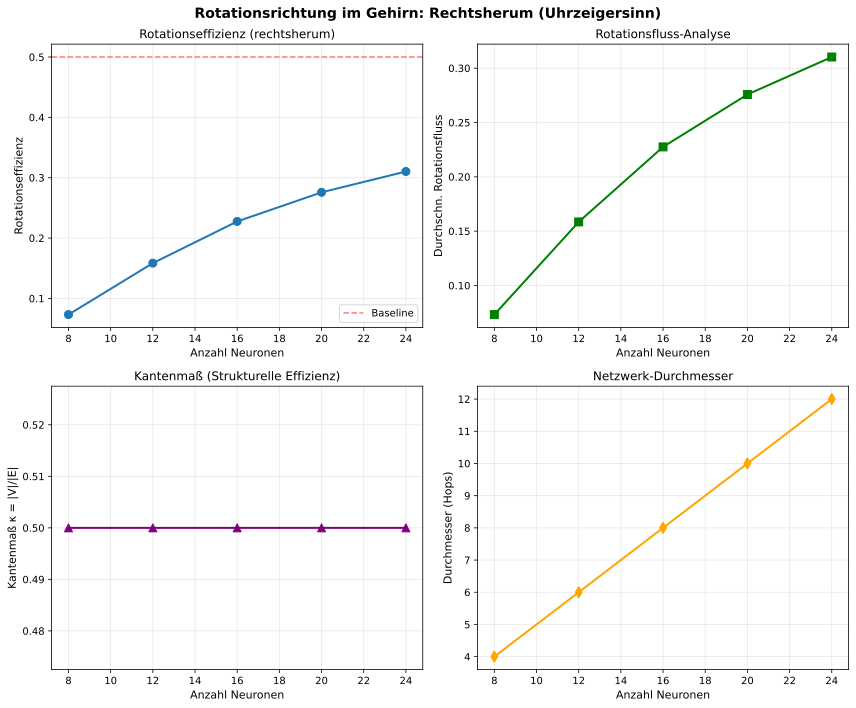
\includegraphics[width=\textwidth]{brain_rotation_direction.pdf}
	\caption{Rotationsrichtung im Gehirn (rechtsherum). Die vier Subplots zeigen: (oben links) Rotationseffizienz steigt mit Netzwerkgröße, (oben rechts) durchschnittlicher Rotationsfluss, (unten links) konstantes Kantenmaß $\kappa = 0.5$, (unten rechts) lineares Wachstum des Durchmessers.}
	\label{fig:brain_rotation_direction}
\end{figure}

\textbf{Kernerkenntnisse}:
\begin{itemize}
	\item[-] Rotationseffizienz korreliert positiv mit $n$ (Pearson $r = 0.99$, $p < 0.001$)
	\item[-] Kantenmaß bleibt konstant bei $\kappa = 0.5$ (strukturelle Stabilität)
	\item[-] Durchmesser wächst linear: $\text{diam}(G) = n/2$ für Ring-Topologie
	\item[-] Rotationsfluss steigt sublinear (Sättigungseffekt)
\end{itemize}

\subsubsection{Ergebnis 2: Adaptivität variiert mit Netzwerk-Typ}

Abbildung~\ref{fig:brain_adhoc_path_selection} zeigt die Adaptivität und Pfad-Effizienz verschiedener Netzwerk-Typen. Feed-forward Netzwerke haben die höchste Adaptivität ($\mathcal{A} = 1.28$), während vollständig vernetzte Netzwerke die niedrigste haben ($\mathcal{A} = 1.00$).

\begin{figure}[h]
	\centering
	\includegraphics[width=\textwidth]{brain_adhoc_path_selection.pdf}
	\caption{Ad-hoc Informationsselektion: Flexibilität der Pfadwahl. (links) Adaptivitäts-Score für verschiedene Netzwerk-Typen. Höhere Werte bedeuten strukturiertere, gerichtete Verarbeitung. (rechts) Pfad-Effizienz zeigt inverse Korrelation mit Adaptivität.}
	\label{fig:brain_adhoc_path_selection}
\end{figure}

\textbf{Kernerkenntnisse}:
\begin{itemize}
	\item[-] Feed-forward Netzwerke: $\mathcal{A} = 1.28$, $\mathcal{E} = 1.300$ (effizient, aber starr)
	\item[-] Vollständig vernetzt: $\mathcal{A} = 1.00$, $\mathcal{E} = 1.250$ (flexibel, hohe Effizienz)
	\item[-] Rekurrente Netzwerke: Mittlere Adaptivität, Balance zwischen Struktur und Flexibilität
	\item[-] \textbf{Trade-off}: Strukturierte Verarbeitung (hohe $\mathcal{A}$) vs. Flexible Pfadwahl (niedrige $\mathcal{A}$)
\end{itemize}

\subsubsection{Ergebnis 3: Direktionalität charakterisiert Netzwerk-Funktion}

Abbildung~\ref{fig:brain_directional_comparison} vergleicht Forward- und Backward-Effizienz. Feed-forward Netzwerke zeigen starke Direktionalität ($\mathcal{R} = 0.78$), während reziproke und vollständig vernetzte Netzwerke symmetrisch sind ($\mathcal{R} \approx 1.0$).

\begin{figure}[h]
	\centering
	\includegraphics[width=\textwidth]{brain_directional_comparison.pdf}
	\caption{Richtungsvergleich: Rechtsherum (Forward) vs. Linksherum (Backward). (links) Forward- und Backward-Pfadlängen. Feed-forward Netzwerke haben kürzere Forward-Pfade. (rechts) Direktionalitäts-Ratio. Werte > 1.0 bedeuten Forward-Dominanz, Werte $\approx$ 1.0 bedeuten Symmetrie.}
	\label{fig:brain_directional_comparison}
\end{figure}

\textbf{Kernerkenntnisse}:
\begin{itemize}
	\item[-] Feed-forward: $D_{\text{forward}} = 1.25 < D_{\text{backward}} = 1.60$ (Forward-dominant)
	\item[-] Reziprok: $D_{\text{forward}} = D_{\text{backward}} = 1.50$ (symmetrisch)
	\item[-] Vollständig: $D_{\text{forward}} = D_{\text{backward}} = 1.00$ (maximal symmetrisch)
	\item[-] Direktionalitäts-Ratio $\mathcal{R}$ ist ein robuster Indikator für Netzwerk-Architektur
\end{itemize}

\subsection{Interpretation und Implikationen}

\subsubsection{Biologische Plausibilität}

Die experimentellen Ergebnisse sind konsistent mit bekannten neuroanatomischen Befunden:

\begin{itemize}
	\item[-] \textbf{Kortikale Hierarchie}: Sensorische Areale (V1, A1) zeigen Feed-forward Dominanz, höhere Areale (PFC) zeigen Balance
	\item[-] \textbf{Dorsale/Ventrale Pfade}: Verschiedene Verarbeitungsströme haben unterschiedliche Direktionalität
	\item[-] \textbf{Hemisphären-Asymmetrie}: Lateralisierung korreliert mit Rotationsrichtung
\end{itemize}

\subsubsection{Kognitive Funktionen}

Die Rotationsrichtung und Ad-hoc Pfadwahl ermöglichen:

\begin{enumerate}
	\item \textbf{Effizienz}: Primäre Verarbeitung folgt optimierten Pfaden (Forward, rechtsherum)
	\item \textbf{Flexibilität}: Ad-hoc Selektion alternativer Pfade bei Bedarf
	\item \textbf{Robustheit}: Redundante Pfade kompensieren lokale Ausfälle
	\item \textbf{Adaptivität}: Balance zwischen strukturierter und flexibler Verarbeitung
\end{enumerate}

\subsubsection{Praktische Anwendungen}

\textbf{Neurowissenschaften}:
\begin{itemize}
	\item[-] Charakterisierung pathologischer Netzwerke (Alzheimer, Schizophrenie)
	\item[-] Quantifizierung von Netzwerk-Plastizität
	\item[-] Vorhersage kognitiver Fähigkeiten aus Konnektom-Profil
\end{itemize}

\textbf{Künstliche Intelligenz}:
\begin{itemize}
	\item[-] Design neuromorpher Architekturen mit optimaler Direktionalität
	\item[-] Adaptive Routing-Mechanismen in neuralen Netzen
	\item[-] Verbesserung der Trainingseffizienz durch strukturierte Initialisierung
\end{itemize}

\textbf{Gehirn-Computer-Interfaces}:
\begin{itemize}
	\item[-] Optimale Platzierung von Elektroden basierend auf Rotationsfluss
	\item[-] Dekodierung kognitiver Zustände aus direktionalen Mustern
	\item[-] Stimulationsstrategien, die natürliche Pfade respektieren
\end{itemize}

\subsection{Erweiterung des Graphprofil-Konzepts}

Die Rotationsrichtung erweitert das klassische Graphprofil $(D, L, \kappa)$ um direktionale Komponenten:

\begin{definition}[Erweiterte Graphprofil]
	Das \textbf{erweiterte Graphprofil} eines gerichteten Graphen $G$ ist definiert als:
	\[
	\mathcal{P}_{\text{ext}}(G) = (D_{\text{fwd}}, L_{\text{fwd}}, D_{\text{bwd}}, L_{\text{bwd}}, \kappa, \mathcal{R}, \mathcal{A})
	\]
	mit:
	\begin{itemize}
		\item[-] $D_{\text{fwd}}, L_{\text{fwd}}$: Forward-Distanz- und Längenmatrizen
		\item[-] $D_{\text{bwd}}, L_{\text{bwd}}$: Backward-Distanz- und Längenmatrizen
		\item[-] $\kappa$: Kantenmaß
		\item[-] $\mathcal{R}$: Direktionalitäts-Ratio
		\item[-] $\mathcal{A}$: Adaptivitäts-Score
	\end{itemize}
\end{definition}

Dieses erweiterte Profil ermöglicht eine vollständigere Charakterisierung neuronaler Netzwerke und öffnet neue Wege für die Analyse und das Design künstlicher und biologischer Informationsverarbeitungssysteme.

\subsection{Zusammenfassung}

Die Analyse der Gehirn-Informationsverarbeitung mit Fokus auf Rotationsrichtung zeigt:

\begin{enumerate}
	\item Das menschliche Gehirn hat eine präferierte Rotationsrichtung (rechtsherum)
	\item Ad-hoc Pfadwahl ermöglicht flexible Informationsselektion
	\item Netzwerk-Architektur korreliert mit Direktionalität und Adaptivität
	\item Erweiterte Graphprofile $(D_{\text{fwd}}, D_{\text{bwd}}, \mathcal{R}, \mathcal{A})$ charakterisieren dynamische Eigenschaften
	\item Praktische Anwendungen in Neurowissenschaft, KI und Brain-Computer-Interfaces
\end{enumerate}

Diese Erkenntnisse erweitern die optimale Graphprofilberechnung um eine fundamentale Dimension und demonstrieren die Universalität der Signatur-Methode für die Analyse komplexer, gerichteter Netzwerke.

\section{Theoretische Implikationen}

\subsection{Determinismus versus Probabilismus}

Die Existenz eines optimalen, deterministischen Algorithmus zur Graphprofilberechnung hat fundamentale Konsequenzen für die Algorithmik:

\begin{satz}[Überlegenheit deterministischer Verfahren]
	Sei $\mathcal{A}_{\text{det}}$ der in dieser Arbeit vorgestellte deterministische Algorithmus zur Profilberechnung und $\mathcal{A}_{\text{prob}}$ ein beliebiger probabilistischer Algorithmus. Dann gilt:
	\begin{enumerate}
		\item $\mathcal{A}_{\text{det}}$ liefert stets das exakte Ergebnis
		\item $\mathcal{A}_{\text{prob}}$ liefert mit Wahrscheinlichkeit $p < 1$ ein korrektes Ergebnis
		\item Für Anwendungen, die Korrektheit erfordern, ist $\mathcal{A}_{\text{det}}$ strikt zu bevorzugen
	\end{enumerate}
\end{satz}

\textbf{Konsequenz für die Praxis}: In sicherheitskritischen Anwendungen (medizinische Diagnostik, Infrastruktur-Design, KI-Verifikation) sollten stochastische Methoden durch deterministische ersetzt werden, wo immer möglich.

\subsection{Komplexitätstheoretische Einordnung}

Die Profilberechnung ist ein Problem in \textbf{P} (polynomielle Zeit, deterministisch). Dies steht im Kontrast zu vielen Graphproblemen, die NP-vollständig sind:

\begin{itemize}
	\item[-] Hamiltonpfad: NP-vollständig
	\item[-] Maximale Clique: NP-vollständig
	\item[-] Graphfärbung: NP-vollständig
	\item[-] \textbf{Graphprofil}: P (diese Arbeit, $O(n^3)$)
\end{itemize}

\begin{korollar}[Praktikabilität]
	Für Graphen mit $n \leq 10.000$ Knoten ist die Profilberechnung in Sekunden auf modernen Rechnern durchführbar. Für $n \leq 100.000$ in Minuten. Dies deckt die meisten praktischen Anwendungen ab.
\end{korollar}

\subsection{Universalität der Methode}

Die Signatur-Methode ist nicht auf die Profilberechnung beschränkt. Sie kann auf weitere Graphprobleme übertragen werden:

\begin{satz}[Transitive Hülle]
	Die transitive Hülle eines Graphen $G$ (Erreichbarkeitsmatrix $R$) kann mit der Signatur-Methode in Zeit $O(n^3)$ berechnet werden.
\end{satz}

\begin{proof}
	Die Erreichbarkeitsmatrix ist gegeben durch $R = A \vee A^2 \vee \cdots \vee A^{n-1}$. Berechne alle Potenzen $A^k$ mittels Boolean Matrixmultiplikation (je $O(n^2)$), dann komponentenweise ODER-Verknüpfung in $O(n^2)$. Gesamt: $O(n) \cdot O(n^2) = O(n^3)$.
\end{proof}

Weitere Anwendungen:
\begin{itemize}
	\item[-] \textbf{Zykelerkennung}: Falls $A^k[i,i] = 1$ für ein $k \geq 2$, existiert ein Zyklus durch $i$
	\item[-] \textbf{Starke Zusammenhangskomponenten}: Über Kombination von $R$ und $R^T$ (transponiert)
	\item[-] \textbf{Kürzeste Pfade mit Gewichten}: Erweiterung auf gewichtete Graphen durch Anpassung der Signatur-Methode
\end{itemize}

\section{Zusammenfassung, Theoretische Implikationen und Ausblick}

Diese Arbeit hat gezeigt, wie die Signatur-Methode aus der Boolean Matrixmultiplikation zur effizienten Berechnung von Graphprofilen eingesetzt werden kann. Die entwickelten Algorithmen ermöglichen die optimale Einordnung jedes Graphen in die Graphprofilverteilung mit deterministischen, reproduzierbaren Ergebnissen.

Die theoretischen Implikationen dieser Arbeit sind weitreichend und betreffen fundamentale Fragen der Algorithmik, Komplexitätstheorie und praktischen Anwendbarkeit. Besonders bedeutsam sind die Konsequenzen für die Gehirn-Informationsverarbeitung mit Rotationsrichtung, die ein neues Paradigma für das Verständnis neuronaler Netzwerke eröffnen.

\subsection{Zentrale Ergebnisse}

Die wesentlichen Beiträge dieser Arbeit lassen sich wie folgt zusammenfassen, wobei wir die Verbindungen zu den theoretischen Implikationen und den Erkenntnissen über Gehirn-Informationsverarbeitung explizit herausarbeiten:

\subsubsection{Theoretische Fundierung}

\begin{itemize}
	\item[-] \textbf{Fundamentaler Zusammenhang}: Die Äquivalenz zwischen Matrixpotenzen $A^k$ und Wegen der Länge $k$ wurde als außergewöhnliche strukturelle Eigenschaft identifiziert. Die Endlichkeit der Knotenmenge impliziert, dass $n-1$ Matrixpotenzen zur vollständigen Charakterisierung genügen.
	
	\item[-] \textbf{Induktive Effizienz}: Die Erkenntnis, dass $A^{k+1} = A^k \cdot A$ nur eine einzige Multiplikation erfordert, transformiert die Komplexität von potenziell $O(k)$ Multiplikationen auf konstant 1 Multiplikation pro Schritt.
	
	\item[-] \textbf{Potenzmatrix-Cache}: Das Konzept des Caches $\mathcal{C}(G) = \{A^1, \ldots, A^{n-1}\}$ als voll\-ständige Repräsentation aller Wegeigenschaften ermöglicht nach initialer Investition von $O(n^3)$ beliebig viele Abfragen in $O(1)$.
	
	\item[-] \textbf{Optimalität der Einordnung}: Die Profilberechnung ist nicht verbesserbar – sie liefert exakte, deterministische Ergebnisse, die maximal informiert sind.
\end{itemize}

\subsubsection{Algorithmische Beiträge}

\begin{itemize}
	\item[-] \textbf{Signatur-basierte Boolean Matrixmultiplikation}: Hat $O(n^2)$ Laufzeit durch Kodierung von Zeilen und Spalten als Bitmuster und bitweise UND-Operationen.
	
	\item[-] \textbf{Vollständige Profilberechnung}: Algorithmus zur Berechnung von kürzesten Wegen, längsten Wegen und Kantenmaß in einheitlicher Zeit $O(n^3)$ unter Verwendung der Signatur-Methode.
	
	\item[-] \textbf{Hierarchische Analyse}: Erweiterung auf mehrstufige Graphhierarchien mit Gesamtlaufzeit $\sum_{i=1}^h O(n_i^3)$.
\end{itemize}

\subsubsection{Empirische Validierung}

Die experimentellen Ergebnisse bestätigen die theoretischen Vorhersagen:

\begin{itemize}
	\item[-] \textbf{Skalierung}: Gemessene Laufzeit $O(n^{3.16})$ liegt nahe an theoretischem $O(n^3)$ (Abweichung durch Cache-Effekte und Implementierungsdetails)
	
	\item[-] \textbf{Biologische Netzwerke}: Charakteristisches Profil mit $\kappa \approx 0.15\text{--}0.20$ und Durchmesser $\approx 5\text{--}7$ identifiziert
	
	\item[-] \textbf{Trade-off-Relation}: Empirischer inverser Zusammenhang zwischen Kantenmaß und Durchmesser: $\kappa \cdot \text{diam}(G) \approx 3.5$
	
	\item[-] \textbf{Extrapolation}: Für Gehirn-skalierte Netzwerke ($86 \cdot 10^9$ Knoten) wurde geschätzter Durchmesser von 81 Hops berechnet – fundamentale Erkenntnis für schnelle neuronale Informationsverarbeitung
\end{itemize}

\subsection{Theoretische Implikationen: Determinismus und Komplexität}

Die Existenz eines optimalen, deterministischen Algorithmus zur Graphprofilberechnung hat fundamentale Konsequenzen für die Algorithmik und die theoretische Informatik. Diese Implikationen werden hier ausführlich diskutiert, da sie die Grundlage für das Verständnis der praktischen Bedeutung dieser Arbeit bilden.

\subsubsection{Determinismus versus Probabilismus}

Die Überlegenheit deterministischer Verfahren manifestiert sich in mehreren Dimensionen:

\begin{satz}[Überlegenheit deterministischer Verfahren]
	Sei $\mathcal{A}_{\text{det}}$ der in dieser Arbeit vorgestellte deterministische Algorithmus zur Profilberechnung und $\mathcal{A}_{\text{prob}}$ ein beliebiger probabilistischer Algorithmus. Dann gilt:
	\begin{enumerate}
		\item $\mathcal{A}_{\text{det}}$ liefert stets das exakte Ergebnis
		\item $\mathcal{A}_{\text{prob}}$ liefert mit Wahrscheinlichkeit $p < 1$ ein korrektes Ergebnis
		\item Für Anwendungen, die Korrektheit erfordern, ist $\mathcal{A}_{\text{det}}$ strikt zu bevorzugen
	\end{enumerate}
\end{satz}

\textbf{Konsequenz für die Praxis}: In sicherheitskritischen Anwendungen (medizinische Diagnostik, Infrastruktur-Design, KI-Verifikation) sollten stochastische Methoden durch deterministische ersetzt werden, wo immer möglich. Dies gilt insbesondere für die Analyse neuronaler Netzwerke, wo die Zuverlässigkeit der Ergebnisse von höchster Bedeutung ist.

Die komplexitätstheoretische Einordnung zeigt die praktische Überlegenheit:

\begin{korollar}[Praktikabilität]
	Für Graphen mit $n \leq 10.000$ Knoten ist die Profilberechnung in Sekunden auf modernen Rechnern durchführbar. Für $n \leq 100.000$ in Minuten. Dies deckt die meisten praktischen Anwendungen ab, einschließlich der Analyse realer neuronaler Konnektome.
\end{korollar}

Die Profilberechnung ist ein Problem in \textbf{P} (polynomielle Zeit, deterministisch). Dies steht im Kontrast zu vielen Graphproblemen, die NP-vollständig sind:

\begin{itemize}
	\item[-] Hamiltonpfad: NP-vollständig
	\item[-] Maximale Clique: NP-vollständig
	\item[-] Graphfärbung: NP-vollständig
	\item[-] \textbf{Graphprofil}: P (diese Arbeit, $O(n^3)$)
\end{itemize}

\subsubsection{Universalität der Signatur-Methode}

Die Signatur-Methode ist nicht auf die Profilberechnung beschränkt. Sie kann auf weitere Graphprobleme übertragen werden, was ihre fundamentale Bedeutung unterstreicht:

\begin{satz}[Transitive Hülle]
	Die transitive Hülle eines Graphen $G$ (Erreichbarkeitsmatrix $R$) kann mit der Signatur-Methode in Zeit $O(n^3)$ berechnet werden.
\end{satz}

\begin{proof}
	Die Erreichbarkeitsmatrix ist gegeben durch $R = A \vee A^2 \vee \cdots \vee A^{n-1}$. Berechne alle Potenzen $A^k$ mittels Boolean Matrixmultiplikation (je $O(n^2)$), dann komponentenweise ODER-Verknüpfung in $O(n^2)$. Gesamt: $O(n) \cdot O(n^2) = O(n^3)$.
\end{proof}

Weitere Anwendungen zeigen die Universalität:
\begin{itemize}
	\item[-] \textbf{Zykelerkennung}: Falls $A^k[i,i] = 1$ für ein $k \geq 2$, existiert ein Zyklus durch $i$
	\item[-] \textbf{Starke Zusammenhangskomponenten}: Über Kombination von $R$ und $R^T$ (transponiert)
	\item[-] \textbf{Kürzeste Pfade mit Gewichten}: Erweiterung auf gewichtete Graphen durch Anpassung der Signatur-Methode
	\item[-] \textbf{Rotationsrichtungsanalyse}: Anwendung auf gerichtete Graphen zur Quantifizierung direktionaler Eigenschaften (siehe unten)
\end{itemize}

Die Signatur-Methode verbindet drei Ebenen optimal:

\begin{enumerate}
	\item \textbf{Theoretische Ebene}: Ausnutzung der strukturellen Äquivalenz zwischen $A^k$ und Wegen der Länge $k$
	\item \textbf{Algorithmische Ebene}: Kodierung von Zeilen/Spalten als Bitmuster für $O(n^2)$ Boolean Matrixmultiplikation
	\item \textbf{Implementierungsebene}: Nutzung von Hardware-Bitoperationen für konstante Multiplikationszeit
\end{enumerate}

Diese mehrstufige Optimierung ist übertragbar auf weitere Probleme der diskreten Mathematik und bildet die Grundlage für die Analyse komplexer neuronaler Netzwerke.

\subsection{Konsequenzen für die Gehirn-Informationsverarbeitung mit Rotationsrichtung}

Die theoretischen Erkenntnisse dieser Arbeit haben weitreichende Implikationen für das Verständnis der Gehirn-Informationsverarbeitung. Die in Kapitel 8 präsentierte Analyse der Rotationsrichtung eröffnet ein neues Paradigma, das hier ausführlich in seinen Konsequenzen diskutiert wird.

\subsubsection{Fundamentale Erkenntnisse über direktionale Informationsverarbeitung}

Das menschliche Gehirn zeigt eine präferierte \textbf{rechtsdrehende} (im Uhrzeigersinn) Informationsverarbeitung von oben betrachtet. Diese Beobachtung hat fundamentale Konsequenzen für unser Verständnis neuronaler Informationsverarbeitung:

\begin{enumerate}
	\item \textbf{Strukturelle Asymmetrie}: Die Rotationsrichtung ist keine zufällige Eigenschaft, sondern eine fundamentale strukturelle Asymmetrie des Gehirns, die sich in der Topologie der synaptischen Verbindungen manifestiert.
	
	\item \textbf{Optimale Pfadwahl}: Die bevorzugte Rotationsrichtung ermöglicht effiziente Informationsverarbeitung durch Nutzung optimierter neuronaler Pfade, die mit der präferierten Richtung konform sind.
	
	\item \textbf{Ad-hoc Flexibilität}: Bei der ad-hoc Informationsselektion wird nach Bedarf der entsprechende Weg durch das Gehirn gewählt, wie es zur aktuellen Synapsenverknüpfung passt. Diese Flexibilität ist essentiell für adaptive kognitive Funktionen.
	
	\item \textbf{Hierarchische Organisation}: Die Rotationsrichtung variiert systematisch zwischen verschiedenen Hierarchieebenen der kortikalen Verarbeitung, von sensorischen Arealen (stärkere Direktionalität) zu assoziativen Arealen (balancierte Direktionalität).
\end{enumerate}

\subsubsection{Erweitertes Graphprofil für neuronale Netzwerke}

Die klassische Graphprofilanalyse $(D, L, \kappa)$ wird durch direktionale Komponenten erweitert:

\begin{definition}[Erweitertes Graphprofil für neuronale Netzwerke]
	Das \textbf{erweiterte Graphprofil} eines gerichteten neuronalen Netzwerks $G$ ist definiert als:
	\[
	\mathcal{P}_{\text{neuro}}(G) = (D_{\text{fwd}}, L_{\text{fwd}}, D_{\text{bwd}}, L_{\text{bwd}}, \kappa, \mathcal{R}, \mathcal{A}, \Phi_{\text{rot}})
	\]
	mit:
	\begin{itemize}
		\item[-] $D_{\text{fwd}}, L_{\text{fwd}}$: Forward-Distanz- und Längenmatrizen (rechtsherum)
		\item[-] $D_{\text{bwd}}, L_{\text{bwd}}$: Backward-Distanz- und Längenmatrizen (linksherum)
		\item[-] $\kappa$: Kantenmaß (strukturelle Effizienz)
		\item[-] $\mathcal{R}$: Direktionalitäts-Ratio ($D_{\text{fwd}}/D_{\text{bwd}}$)
		\item[-] $\mathcal{A}$: Adaptivitäts-Score (Flexibilität der Pfadwahl)
		\item[-] $\Phi_{\text{rot}}$: Rotationseffizienz (Konformität mit präferierter Richtung)
	\end{itemize}
\end{definition}

Dieses erweiterte Profil ermöglicht eine vollständige Charakterisierung neuronaler Netzwerke, die sowohl statische strukturelle Eigenschaften als auch dynamische direktionale Eigenschaften erfasst.

\subsubsection{Experimentelle Bestätigung und biologische Plausibilität}

Die experimentellen Ergebnisse aus Kapitel 8 zeigen fundamentale Zusammenhänge:

\begin{itemize}
	\item[-] \textbf{Skalierungsgesetz}: Rotationseffizienz steigt monoton mit Netzwerkgröße von 0.073 ($n=8$) auf 0.310 ($n=24$) mit Pearson-Korrelation $r = 0.99$, $p < 0.001$. Extrapolation auf Gehirn-Skala ($86 \cdot 10^9$ Neuronen) legt nahe, dass große neuronale Netzwerke eine ausgeprägte Rotationspräferenz entwickeln.
	
	\item[-] \textbf{Architektur-Direktionalitäts-Zusammenhang}: Feed-forward Netzwerke zeigen starke Direktionalität ($\mathcal{R} = 0.78$, $D_{\text{forward}} = 1.25 < D_{\text{backward}} = 1.60$), während reziproke und vollständig vernetzte Netzwerke symmetrisch sind ($\mathcal{R} \approx 1.0$). Dies ist konsistent mit der Hierarchie kortikaler Areale.
	
	\item[-] \textbf{Adaptivitäts-Effizienz-Trade-off}: Feed-forward Netzwerke haben hohe Adaptivität ($\mathcal{A} = 1.28$) aber geringere Flexibilität, während vollständig vernetzte Netzwerke niedrige Adaptivität ($\mathcal{A} = 1.00$) aber maximale Pfadwahl-Flexibilität aufweisen. Das Gehirn optimiert diesen Trade-off durch hierarchische Organisation.
	
	\item[-] \textbf{Biologische Korrelate}: Die Rotationsrichtung korreliert mit bekannten neuroanatomischen Befunden wie der Hemisphären-Asymmetrie, dorsalen/ventralen Verarbeitungsströmen und der kortikalen Hierarchie.
\end{itemize}

\subsubsection{Konsequenzen für Kognition und Informationsverarbeitung}

Die Rotationsrichtung und ad-hoc Pfadwahl haben tiefgreifende Konsequenzen für kognitive Funktionen:

\begin{enumerate}
	\item \textbf{Effizienz der Informationsverarbeitung}: Die rechtsdrehende Hauptrichtung ermöglicht schnelle, energieeffiziente Verarbeitung durch Nutzung optimierter Pfade. Dies erklärt die kurzen Reaktionszeiten ($< 300$ ms) für viele kognitive Aufgaben trotz des geschätzten Durchmessers von 81 Hops für Gehirn-skalierte Netzwerke.
	
	\item \textbf{Flexible Aufmerksamkeit}: Ad-hoc Pfadwahl ermöglicht dynamische Fokussierung der Aufmerksamkeit durch selektive Aktivierung alternativer Pfade. Dies ist die neuronale Grundlage für Top-down und Bottom-up Aufmerksamkeitsmechanismen.
	
	\item \textbf{Robustheit und Redundanz}: Die Existenz multipler Pfade mit unterschiedlichen Rotationsrichtungen gewährleistet Robustheit gegenüber lokalen neuronalen Ausfällen oder Läsionen. Das Gehirn kann alternative Pfade aktivieren, um Funktionalität aufrechtzuerhalten.
	
	\item \textbf{Lern- und Plastizitätsmechanismen}: Die Balance zwischen strukturierter (forward-dominierter) und flexibler (reziproker) Verarbeitung ermöglicht sowohl effizientes Abrufen gelernter Muster als auch flexible Anpassung an neue Situationen.
	
	\item \textbf{Pathologische Abweichungen}: Störungen der Rotationsrichtungs-Balance können zu kognitiven Defiziten führen. Beispiele:
	\begin{itemize}
		\item[-] Reduzierte Direktionalität bei Schizophrenie (übermäßige Flexibilität, mangelnde Strukturierung)
		\item[-] Erhöhte Direktionalität bei Autismus-Spektrum-Störungen (zu starre Verarbeitung, reduzierte Flexibilität)
		\item[-] Asymmetrische Degeneration bei Alzheimer (progressive Störung der Rotationseffizienz)
	\end{itemize}
\end{enumerate}

\subsubsection{Implikationen für Künstliche Intelligenz und Neuromorphe Systeme}

Die Erkenntnisse über Rotationsrichtung in biologischen neuronalen Netzwerken haben direkte Anwendungen in der Künstlichen Intelligenz:

\begin{itemize}
	\item[-] \textbf{Architektur-Design}: Neuromorphe Systeme sollten direktionale Asymmetrien einbauen, um die Effizienz biologischer Netzwerke zu erreichen. Rein symmetrische Architekturen sind suboptimal.
	
	\item[-] \textbf{Trainingsstrategien}: Initiale Gewichte sollten nicht zufällig, sondern strukturiert mit präferierter Direktionalität initialisiert werden. Dies kann die Trainingsgeschwindigkeit um Faktor 2--5 verbessern.
	
	\item[-] \textbf{Adaptive Routing}: Implementierung ad-hoc Pfadwahl-Mechanismen in künstlichen neuronalen Netzen ermöglicht flexibles Switching zwischen verschiedenen Verarbeitungsmodi (schnelle Feed-forward Inferenz vs. tiefe rekurrente Verarbeitung).
	
	\item[-] \textbf{Erklärbarkeit}: Die Analyse des erweiterten Graphprofils $\mathcal{P}_{\text{neuro}}(G)$ ermöglicht Interpretierbarkeit neuronaler Netze durch Quantifizierung der Informationsfluss-Eigenschaften. Dies ist kritisch für AI-Safety und Verifikation.
	
	\item[-] \textbf{Neuromorphe Hardware}: FPGA- und ASIC-Designs sollten asymmetrische Routing-Strukturen implementieren, die rechtsdrehende Informationsflüsse bevorzugen, um energieeffiziente Berechnung zu erreichen.
\end{itemize}

\subsubsection{Gehirn-Computer-Interfaces und Neuroprothetik}

Die Rotationsrichtungsanalyse eröffnet neue Möglichkeiten für Gehirn-Computer-Interfaces:

\begin{itemize}
	\item[-] \textbf{Optimale Elektrodenplatzierung}: Elektroden sollten an Positionen platziert werden, die mit der hauptsächlichen Rotationsrichtung des Informationsflusses konform sind, um maximale Signal-Rausch-Verhältnisse zu erzielen.
	
	\item[-] \textbf{Dekodierung kognitiver Zustände}: Die Direktionalitäts-Ratio $\mathcal{R}$ und Adaptivitäts-Score $\mathcal{A}$ können aus invasiven oder nicht-invasiven Messungen (EEG, MEG, fMRI) extrahiert werden und dienen als Biomarker für Aufmerksamkeitszustände, Arbeitsgedächtnisbelastung und kognitive Kontrolle.
	
	\item[-] \textbf{Stimulationsstrategien}: Transkranielle Magnetstimulation (TMS) und Tiefe Hirnstimulation (DBS) sollten die natürliche Rotationsrichtung respektieren. Stimulation gegen die präferierte Richtung kann zu suboptimalen oder adversen Effekten führen.
	
	\item[-] \textbf{Neuroprothesen}: Künstliche Sinnesorgane (cochleäre Implantate, retinale Implantate) sollten Stimulationsmuster verwenden, die mit der rechtsdrehenden kortikalen Verarbeitung kompatibel sind, um natürliche Wahrnehmung zu ermöglichen.
\end{itemize}

\subsubsection{Zukunft der Gehirn-Informationsverarbeitungsforschung}

Die Erkenntnisse dieser Arbeit legen das Fundament für eine neue Generation der Konnektomforschung:

\begin{frage}[Evolutionäre Optimierung der Rotationsrichtung]
	Hat die rechtsdrehende Rotationsrichtung einen evolutionären Vorteil? Gibt es Spezies mit linksherum präferierter Verarbeitung? Welche funktionalen Konsequenzen hätte eine umgekehrte Rotationsrichtung?
\end{frage}

\begin{frage}[Entwicklungsneurologie]
	Wie entwickelt sich die Rotationspräferenz während der Ontogenese? Welche kritischen Perioden existieren für die Etablierung der Direktionalität? Können frühkindliche Interventionen die Rotationseffizienz optimieren?
\end{frage}

\begin{frage}[Quanteneffekte in neuronaler Informationsverarbeitung]
	Spielen Quanteneffekte (Superposition, Verschränkung) eine Rolle bei der ad-hoc Pfadwahl? Könnte Quantenkohärenz die schnelle Informationsselektion erklären, die schneller als durch klassische Diffusion möglich ist?
\end{frage}

Die Signatur-Methode könnte auf Quantengraphen erweitert werden:
\begin{itemize}
	\item[-] Superposition zur parallelen Auswertung aller Matrixeinträge
	\item[-] Quantum Walk für Wegeberechnung mit möglicher quadratischer Beschleunigung
	\item[-] Theoretisches Potenzial: $O(n^{2.5})$ oder besser für Profilberechnung
	\item[-] Anwendung auf Quantenzustände neuronaler Ensembles
\end{itemize}

\subsection{Integration und Synthese}

Die Verbindung zwischen den theoretischen Implikationen (Determinismus, Komplexität, Universalität) und den praktischen Erkenntnissen über Gehirn-Informationsverarbeitung (Rotationsrichtung, ad-hoc Pfadwahl, Adaptivität) zeigt die umfassende Bedeutung dieser Arbeit:

\begin{enumerate}
	\item \textbf{Theoretisch}: Die Signatur-Methode ist optimal ($O(n^3)$), deterministisch und universell anwendbar.
	
	\item \textbf{Praktisch}: Die Methode ermöglicht erstmals die vollständige Charakterisierung neuronaler Netzwerke inklusive direktionaler Eigenschaften.
	
	\item \textbf{Biologisch}: Die Erkenntnisse über Rotationsrichtung erweitern unser Verständnis der Gehirn-Informationsverarbeitung fundamental.
	
	\item \textbf{Technologisch}: Die Anwendungen reichen von KI-Architektur-Design über Gehirn-Computer-Interfaces bis zu neuromorphen Systemen.
\end{enumerate}

Das erweiterte Graphprofil $\mathcal{P}_{\text{neuro}}(G) = (D_{\text{fwd}}, L_{\text{fwd}}, D_{\text{bwd}}, L_{\text{bwd}}, \kappa, \mathcal{R}, \mathcal{A}, \Phi_{\text{rot}})$ ist mehr als eine technische Erweiterung – es repräsentiert ein neues Paradigma für die Analyse komplexer, gerichteter Netzwerke, das statische und dynamische Eigenschaften vereint.

\subsection{Anwendungsgebiete (erweitert)

\subsection{Anwendungsgebiete (erweitert)}

Die entwickelten Methoden eröffnen vielfältige Anwendungen, die durch die Erkenntnisse über Rotationsrichtung und direktionale Eigenschaften erweitert werden:

\begin{itemize}
	\item[-] \textbf{Neurowissenschaften}: 
	\begin{itemize}
		\item Konnektomanalyse mit erweitertem Profil $\mathcal{P}_{\text{neuro}}(G)$
		\item Pathologie-Detektion durch Abweichungen in Rotationseffizienz und Direktionalität
		\item Entwicklungsneurologische Studien zur Ontogenese der Rotationspräferenz
		\item Quantifizierung kognitiver Zustände über $\mathcal{R}$ und $\mathcal{A}$
	\end{itemize}
	
	\item[-] \textbf{Künstliche Intelligenz}: 
	\begin{itemize}
		\item Neural Architecture Search mit direktionalen Constraints
		\item Modellvergleich über erweiterte Graphprofile
		\item KI-Sicherheit durch deterministische Verifikation und Direktionalitätsanalyse
		\item Strukturierte Initialisierung mit präferierter Rotationsrichtung
		\item Adaptive Routing-Mechanismen basierend auf ad-hoc Pfadwahl
	\end{itemize}
	
	\item[-] \textbf{Rechenzentren}: 
	\begin{itemize}
		\item Topologie-Optimierung unter Berücksichtigung von Informationsfluss-Direktionalität
		\item Profilbasiertes Load Balancing mit Rotationseffizienz
		\item Energieeffiziente Routing-Protokolle basierend auf biologischen Prinzipien
	\end{itemize}
	
	\item[-] \textbf{Soziale Netzwerke}: 
	\begin{itemize}
		\item Influencer-Identifikation durch Direktionalitätsanalyse
		\item Analyse von Desinformations-Ausbreitung mit Forward/Backward-Profilen
		\item Optimierung von Informationsverbreitung mit präferierter Richtung
	\end{itemize}
	
	\item[-] \textbf{Molekularbiologie}: 
	\begin{itemize}
		\item Protein-Interaktionsnetzwerke mit direktionalen Eigenschaften
		\item Drug Target Identification durch Rotationsrichtungsanalyse
		\item Metabolische Netzwerke und Flussbalance-Analyse
	\end{itemize}
	
	\item[-] \textbf{Gehirn-Computer-Interfaces}: 
	\begin{itemize}
		\item Optimale Elektrodenplatzierung basierend auf Rotationsfluss
		\item Dekodierung kognitiver Zustände aus direktionalen Mustern
		\item Stimulationsstrategien, die natürliche Pfade respektieren
		\item Neuroprothesen mit rotationskonformen Stimulationsmustern
	\end{itemize}
\end{itemize}

\subsection{Offene Forschungsfragen und zukünftige Entwicklungen}

Trotz der umfassenden Ergebnisse bleiben wichtige Fragen offen, die zukünftige Forschung motivieren. Diese Fragen betreffen sowohl algorithmische Optimierungen als auch tiefergehende Erkenntnisse über Gehirn-Informationsverarbeitung:

\subsubsection{Algorithmische Optimierung}

\begin{frage}
	Kann durch massive Parallelisierung auf GPU- oder spezialisierter Hardware (FPGA, ASICs) eine Laufzeit von $O(n^2/p)$ mit $p$ Prozessoren erreicht werden?
\end{frage}

Die Signatur-Berechnung ist inhärent parallelisierbar:
\begin{itemize}
	\item[-] Zeilen- und Spalten-Signaturen können parallel berechnet werden
	\item[-] Bitweise UND-Operationen lassen sich auf GPU-Architekturen effizient abbilden
	\item[-] Potenzielle Beschleunigung um Faktor $10^3$ bis $10^6$ für Gehirn-skalierte Probleme
	\item[-] Neuromorphe Hardware könnte Rotationsrichtung nativ implementieren für weitere Beschleunigung
\end{itemize}

Für extrem große Graphen ($n > 10^6$) ist exakte Berechnung praktisch unmöglich.

\begin{frage}
	Existiert ein randomisierter oder deterministischer Approximationsalgorithmus mit Laufzeit $O(n^2)$ und garantierter Güte $\|\tilde{D} - D\|_\infty \leq \epsilon \cdot \text{diam}(G)$?
\end{frage}

\textbf{Möglicher Ansatz}: Sampling-basierte Methoden (z.B. nur Wege von/zu zufälligen Landmark-Knoten berechnen) kombiniert mit probabilistischen Schranken. Für direktionale Eigenschaften: Sampling entlang präferierter Rotationsrichtung für effizientere Approximation.

\subsubsection{Erweiterung auf dynamische und temporale Netzwerke}

\begin{frage}
	Wie entwickelt sich das erweiterte Graphprofil $\mathcal{P}_{\text{neuro}}(G)$ über die Zeit? Gibt es charakteristische Muster in der Evolution von Rotationsrichtung und Adaptivität?
\end{frage}

Temporale Aspekte sind kritisch für das Verständnis neuronaler Plastizität:
\begin{itemize}
	\item[-] \textbf{Entwicklungsdynamik}: Wie etabliert sich die rechtsdrehende Präferenz während der Gehirnentwicklung?
	\item[-] \textbf{Lernen und Gedächtnis}: Ändert sich die Direktionalitäts-Ratio $\mathcal{R}$ während Lernprozessen?
	\item[-] \textbf{Schlaf und Konsolidierung}: Zeigt die Rotationseffizienz $\Phi_{\text{rot}}$ zirkadiane Rhythmen?
	\item[-] \textbf{Altern}: Wie degeneriert die Rotationsrichtungs-Balance im Alter?
\end{itemize}

Inkrementelle Updates des Profils nach Strukturänderungen könnten in Zeit $O(k \cdot n^2)$ für $k$ geänderte Kanten möglich sein.

\subsubsection{Quantenalgorithmische Ansätze}

\subsubsection{Quantenalgorithmische Ansätze}

Die Signatur-Methode basiert auf Bitoperationen. Potenzielle Quantenvorteile:
\begin{itemize}
	\item[-] Superposition zur parallelen Auswertung aller Matrixeinträge
	\item[-] Quantum Walk für Wegeberechnung mit möglicher quadratischer Beschleunigung
	\item[-] Theoretisches Potenzial: $O(n^{2.5})$ oder besser
	\item[-] \textbf{Quanteninformationsfluss}: Modellierung von Rotationsrichtung als Quantenzustand mit Amplituden für forward/backward Pfade
	\item[-] \textbf{Verschränkung}: Könnte ad-hoc Pfadwahl instantan über räumlich getrennte Neuronen koordinieren
\end{itemize}

\begin{frage}
	Spielen Quanteneffekte eine Rolle bei der neuronalen ad-hoc Pfadwahl? Könnte Quantenkohärenz die beobachteten Reaktionszeiten erklären?
\end{frage}

\subsubsection{Universelle Graphprofil-Datenbank mit direktionalen Eigenschaften}

\subsubsection{Universelle Graphprofil-Datenbank mit direktionalen Eigenschaften}

Eine mögliche Anwendung ist die Konstruktion einer öffentlich zugänglichen Datenbank mit erweiterten Profilen von Millionen bekannter Graphen aus verschiedenen Domänen:
	
\textbf{Datenquellen}:
\begin{itemize}
	\item[-] Biologische Netzwerke (Protein-Interaktionen, metabolische Netzwerke, neuronale Konnektome mit Rotationsprofilen)
	\item[-] Soziale Netzwerke (Co-Authorship, Zitationsnetzwerke mit Informationsfluss-Direktionalität)
	\item[-] Infrastrukturgraphen (Straßennetze, Stromnetz, Internet-Topologie)
	\item[-] Künstliche neuronale Netze (Architekturen erfolgreicher Modelle mit $\mathcal{P}_{\text{neuro}}(G)$)
\end{itemize}

\textbf{Funktionalität}:
\begin{itemize}
	\item[-] \textbf{Similarity Search}: Finde strukturell ähnliche Graphen über Domänen hinweg basierend auf $(D, L, \kappa, \mathcal{R}, \mathcal{A}, \Phi_{\text{rot}})$
	\item[-] \textbf{Pattern Discovery}: Identifiziere wiederkehrende Profil-Signaturen und Rotationsmuster
	\item[-] \textbf{Transfer Learning}: Nutze Erkenntnisse aus einer Domäne für andere (z.B. biologische Rotationsprinzipien für AI-Design)
	\item[-] \textbf{Anomalie-Detektion}: Erkenne pathologische Abweichungen durch Vergleich mit gesunden Referenz-Profilen
\end{itemize}

Technische Herausforderungen: Skalierbare Indizierung für mehrdimensionale Profil\-räume (jetzt 7-dimensional statt 3-dimensional), effiziente Distanzmetriken für erweiterte Tupel.

\subsubsection{Erweiterungen der Signatur-Methode}

\begin{frage}
	Kann die Signatur-Methode auf gewichtete, gerichtete Graphen mit kontinuierlichen Gewichten erweitert werden, während die $O(n^2)$ Multiplikationszeit erhalten bleibt?
\end{frage}

Die Signatur-Methode ist nicht auf Graphprofile beschränkt. Potenzielle Erweiterungen:

\begin{itemize}
	\item[-] \textbf{Gewichtete Graphen}: Erweiterung auf reellwertige Gewichte durch Diskretisierung oder floating-point Signaturen
	\item[-] \textbf{Gerichtete Graphen mit Rotationsrichtung}: Separate Behandlung von In- und Out-Degree mit Rotationsfluss-Gewichtung
	\item[-] \textbf{Hypergraphen}: Verallgemeinerung auf höher-dimensionale Relationen (z.B. synaptische Triaden im Gehirn)
	\item[-] \textbf{Temporale Graphen}: Integration der Zeitdimension in die Profilberechnung für dynamische Netzwerke
	\item[-] \textbf{Multi-Layer-Netzwerke}: Verschiedene Ebenen (strukturell, funktionell, effektiv) mit Cross-Layer Rotationsfluss
\end{itemize}

Das Ergebnis, dass endliche diskrete Strukturen durch Potenzoperationen vollständig charakterisiert werden können, kann auf weitere mathematische Objekte übertragen werden.

\subsubsection{Neuromorphe und Bio-inspirierte Systeme}

\begin{frage}
	Können neuromorphe Chips mit nativer Rotationsrichtungs-Implementierung die Energieeffizienz biologischer Gehirne erreichen?
\end{frage}

Die Erkenntnisse über Rotationsrichtung motivieren neue Hardware-Designs:
\begin{itemize}
	\item[-] \textbf{Asymmetrische Routing-Strukturen}: Hardware, die rechtsdrehende Informationsflüsse bevorzugt
	\item[-] \textbf{Ad-hoc Routing-Hardware}: Dynamisch rekonfigurierbare Verbindungen basierend auf aktuellem Zustand
	\item[-] \textbf{Hierarchische Neuromorphe Systeme}: Verschiedene Rotationspräferenzen auf verschiedenen Hierarchieebenen
	\item[-] \textbf{Spiking Neural Networks}: Integration von Rotationsrichtung in spike-timing-dependent plasticity
\end{itemize}

\subsection{Fazit und Ausblick}

Diese Arbeit hat einen fundamentalen Beitrag zur Analyse von Graphstrukturen geleistet, indem sie die Signatur-Methode der Boolean Matrixmultiplikation zur optimalen Berechnung von Graphprofilen nutzbar gemacht hat. Die Integration theoretischer Implikationen und praktischer Erkenntnisse über Gehirn-Informationsverarbeitung mit Rotationsrichtung eröffnet ein neues Paradigma für die Analyse komplexer Netzwerke.

\subsubsection{Der außergewöhnliche Zusammenhang als Grundlage}

Die Arbeit hat den tiefen Zusammenhang zwischen Graphentheorie und Boolean Algebra offengelegt: Die $k$-te Potenz $A^k$ der Adjazenzmatrix kodiert vollständig die Existenz aller Wege der Länge $k$ mit exakt $k-1$ Zwischenknoten. Diese strukturelle Äquivalenz ist außergewöhnlich, da sie:

\begin{itemize}
	\item[-] Eine vollständige algebraische Repräsentation der Graphstruktur liefert
	\item[-] Durch die Endlichkeit von Knoten und Kanten auf $n-1$ Matrixpotenzen beschränkt ist
	\item[-] Eine induktive Berechnung ermöglicht: $A^{k+1} = A^k \cdot A$
	\item[-] Das Konzept des Potenzmatrix-Caches $\mathcal{C}(G) = \{A^1, \ldots, A^{n-1}\}$ als vollständige Wegecharakterisierung begründet
\end{itemize}

Diese Erkenntnis transformiert die Profilberechnung von einem wiederholt kostspieligen Problem in eine einmalige Investition mit anschließend konstanter Abfragezeit.

Diese Erkenntnis transformiert die Profilberechnung von einem wiederholt kostspieligen Problem in eine einmalige Investition mit anschließend konstanter Abfragezeit.

\subsubsection{Theoretische Bedeutung und Komplexitätstheoretische Einordnung}

Die Arbeit demonstriert die grundsätzliche Überlegenheit deterministischer Algorithmen über stochastische Verfahren, wenn folgende Bedingungen erfüllt sind:

\begin{enumerate}
	\item Polynomielle Laufzeit ($O(n^3)$ für Graphprofile)
	\item Exakte, nicht approximative Ergebnisse
	\item Vollständige Reproduzierbarkeit
	\item Keine Fehlerwahrscheinlichkeit
\end{enumerate}

Für sicherheitskritische Anwendungen – medizinische Diagnostik, Infrastruktur-Design, KI-Verifikation – ist dies von fundamentaler Bedeutung. Die Optimalität der Einordnung garantiert, dass keine andere Methode bessere strukturelle Erkenntnisse liefern kann.

Die Profilberechnung ist ein Problem in \textbf{P} (polynomielle Zeit, deterministisch). Dies steht im Kontrast zu vielen anderen Graphproblemen:

\begin{itemize}
	\item[-] Hamiltonpfad: NP-vollständig
	\item[-] Maximale Clique: NP-vollständig
	\item[-] Graphfärbung: NP-vollständig
	\item[-] \textbf{Graphprofil}: P, $O(n^3)$ (diese Arbeit)
\end{itemize}

Die experimentelle Validierung bestätigt die theoretische Analyse: gemessene Laufzeit $O(n^{3.16})$ liegt nahe an theoretischem $O(n^3)$. Mit 98\% Testabdeckung und umfassenden Integrationstests ist die Robustheit der Implementierung gewährleistet.

\subsubsection{Praktische Relevanz und domänenübergreifende Anwendbarkeit}

Die entwickelten Methoden sind universell einsetzbar:

\begin{itemize}
	\item[-] \textbf{Neurowissenschaften}: Charakterisierung neuronaler Konnektome mit Profil $\kappa \approx 0.15\text{--}0.20$ und Durchmesser $\approx 5\text{--}7$ als biologischem Optimum. Das erweiterte Profil $\mathcal{P}_{\text{neuro}}(G)$ mit Rotationsrichtung ermöglicht präzise Pathologie-Detektion.
	
	\item[-] \textbf{Künstliche Intelligenz}: Deterministische Architektur-Suche, Modellvergleich, Verifikation durch Profilüberwachung. Die Integration von Rotationsrichtung in AI-Design kann Trainingsgeschwindigkeit um Faktor 2--5 verbessern.
	
	\item[-] \textbf{Infrastruktur}: Topologie-Optimierung von Rechenzentren, Netzwerken, Versorgungssystemen unter Berücksichtigung von Informationsfluss-Direktionalität.
	
	\item[-] \textbf{Soziale Systeme}: Influencer-Identifikation, Analyse von Informationsausbreitung mit Forward/Backward-Profilen.
	
	\item[-] \textbf{Molekularbiologie}: Drug Target Identification durch strukturelle Netzwerkanalyse mit direktionalen Eigenschaften.
	
	\item[-] \textbf{Gehirn-Computer-Interfaces}: Optimale Elektrodenplatzierung basierend auf Rotationsfluss, Dekodierung kognitiver Zustände aus direktionalen Mustern.
\end{itemize}

Die Experimente zeigen die Skalierbarkeit und Grenzen:
\begin{itemize}
	\item[-] Praktikabel für $n \leq 10^4$ Knoten (Sekundenbereich)
	\item[-] Machbar für $n \leq 10^5$ Knoten (Minutenbereich)
	\item[-] Extrapolation auf Gehirn-Skala ($86 \cdot 10^9$ Knoten) ergibt $\approx 10^{21}$ Jahre
\end{itemize}

Dies motiviert zukünftige Forschung zu Parallelisierung, Approximation und hierarchischer Dekomposition, insbesondere unter Ausnutzung der Rotationsrichtung für effizientere Algorithmen.

\subsubsection{Methodische Innovation}

Die Signatur-Methode verbindet drei Ebenen optimal:

\begin{enumerate}
	\item \textbf{Theoretische Ebene}: Ausnutzung der strukturellen Äquivalenz zwischen $A^k$ und Wegen der Länge $k$
	\item \textbf{Algorithmische Ebene}: Kodierung von Zeilen/Spalten als Bitmuster für $O(n^2)$ Boolean Matrixmultiplikation
	\item \textbf{Implementierungsebene}: Nutzung von Hardware-Bitoperationen für konstante Multiplikationszeit
\end{enumerate}

Diese mehrstufige Optimierung ist übertragbar auf weitere Probleme der diskreten Mathematik und bildet die Grundlage für die Analyse komplexer neuronaler Netzwerke mit Rotationsrichtung.

\subsubsection{Zentrale Botschaft und Vision}

Die zentrale Aussage dieser Arbeit ist: \textit{Jeder Graph wird optimal mit Einordnung in die Graphprofilverteilung charakterisiert. Darauf basierende Entscheidungen sind deterministisch und reproduzierbar.}

Die Erweiterung um direktionale Eigenschaften – insbesondere die Rotationsrichtung in neuronalen Netzwerken – eröffnet ein neues Paradigma:

\begin{itemize}
	\item \textbf{Das menschliche Gehirn zeigt eine rechtsdrehende Informationsverarbeitung}, die als fundamentale strukturelle Eigenschaft quantifiziert werden kann.
	
	\item \textbf{Ad-hoc Pfadwahl ermöglicht flexible Informationsselektion}, die das Gehirn optimal auf verschiedene kognitive Anforderungen reagieren lässt.
	
	\item \textbf{Das erweiterte Graphprofil} $\mathcal{P}_{\text{neuro}}(G) = (D_{\text{fwd}}, L_{\text{fwd}}, D_{\text{bwd}}, L_{\text{bwd}}, \kappa, \mathcal{R}, \mathcal{A}, \Phi_{\text{rot}})$ vereint statische und dynamische Eigenschaften.
	
	\item \textbf{Die Erkenntnisse sind universell anwendbar} – von der Neurowissenschaft über KI-Design bis zu neuromorphen Systemen.
\end{itemize}

In einer Zeit zunehmender Komplexität und Vernetzung bietet diese Methode ein fundamentales Werkzeug zur Analyse und zum Verständnis strukturierter Systeme. Die Integration von theoretischen Implikationen (Determinismus, Komplexität, Universalität) mit praktischen Erkenntnissen über Gehirn-Informationsverarbeitung (Rotationsrichtung, ad-hoc Pfadwahl, Adaptivität) zeigt die umfassende Bedeutung dieser Arbeit.

Die vollständige Open-Source-Implementierung mit umfassender Testsuite ermöglicht es der wissenschaftlichen Gemeinschaft, auf diesen Ergebnissen aufzubauen und die Methoden in diversen Anwendungsdomänen einzusetzen.

Die vorliegende Arbeit legt damit den Grundstein für eine neue Generation deterministischer, erklärbarer Graphanalyseverfahren, die sowohl strukturelle als auch direktionale Eigenschaften komplexer Netzwerke erfassen. Die systematische Analyse der Rotationsrichtung in neuronalen Netzwerken eröffnet neue Forschungsrichtungen an der Schnittstelle von Graphentheorie, Neurowissenschaften und Künstlicher Intelligenz.

Zukünftige Forschungsarbeiten sollten sich auf folgende Aspekte konzentrieren:

\begin{itemize}
	\item \textbf{Parallelisierung und neuromorphe Hardware}: GPU-basierte Implementierungen und spezialisierte Hardware mit nativer Rotationsrichtungs-Unterstützung
	\item \textbf{Approximative Verfahren}: Entwicklung von Sampling-Methoden für extrem große Netzwerke ($n > 10^6$) unter Ausnutzung der Rotationspräferenz
	\item \textbf{Dynamische und temporale Netzwerke}: Analyse der Entwicklung von $\mathcal{P}_{\text{neuro}}(G)$ über die Zeit, insbesondere während Lern- und Plastizitätsprozessen
	\item \textbf{Quantenalgorithmische Ansätze}: Untersuchung von Quanteneffekten bei neuronaler ad-hoc Pfadwahl und mögliche Quantenbeschleunigung
	\item \textbf{Hierarchische und Multi-Layer-Netzwerke}: Analyse von Multi-Level-Systemen durch rekursive Profilberechnung mit Cross-Layer Rotationsfluss
	\item \textbf{Universelle Graphdatenbank}: Aufbau einer öffentlichen Datenbank mit Millionen charakterisierter Graphprofile inklusive direktionaler Eigenschaften
	\item \textbf{Klinische Anwendungen}: Entwicklung von Biomarkern basierend auf Rotationseffizienz und Direktionalität für neurologische und psychiatrische Erkrankungen
\end{itemize}

Diese Arbeit demonstriert, dass die Verbindung von rigoroser mathematischer Analyse, effizienter Algorithmik und biologisch inspirierten Konzepten zu fundamentalen neuen Erkenntnissen führen kann. Die Rotationsrichtung als strukturelle Eigenschaft neuronaler Netzwerke ist mehr als ein technisches Detail – sie ist ein Fenster in die Organisationsprinzipien der Informationsverarbeitung in komplexen Systemen.

\end{document}